\documentclass[a4paper,10pt,twoside]{article}
\usepackage[utf8x]{inputenc}
\usepackage[ngerman]{babel}
\usepackage{cite}
\usepackage{amsmath}
\usepackage{rotating}
\usepackage{graphicx}
\usepackage{epsfig}
\usepackage{hyperref}

\usepackage[percent]{overpic}
\usepackage{color}
\usepackage{subfig}
\usepackage{placeins}
\usepackage{epsfig}
\usepackage{gensymb}
\usepackage{supertabular}
\usepackage{pdfpages}


\usepackage{amsfonts}
\usepackage{amssymb}

\usepackage{pstricks}
\usepackage{pst-plot}
\usepackage[all]{xy}

\hypersetup{
%    bookmarks=true,
    pdftoolbar=true,
    pdfmenubar=true,
    pdffitwindow=false,
    pdfstartview={FitH},
    pdftitle={Die Pioneer-Anomalie},
    pdfauthor={Judith Selig, Michael F. Sch\"onitzer, Florian Schlagintweit},
    pdfsubject={Pioneer-Anomalie},
    pdfkeywords={Pioneer} {Anomalie} {Physik} {Raumfahrt},
    pdfnewwindow=true,
    colorlinks=true,
    linkcolor=black,
    citecolor=black,
    filecolor=black,
    urlcolor=blue
}
\linespread{1.359140914229522617680} 
\usepackage{a4wide}
\setlength{\oddsidemargin}{0cm}
\setlength{\evensidemargin}{1cm}

\newcommand{\rem}[1]{}

%opening
\title{Die Pioneer-Anomalie}
%\author{Judith Selig\footnote{judith.selig@gmx.de}, Michael F. Schönitzer\footnote{michael@schoenitzer.de}, Florian Schlagintweit\footnote{florian@schlagintweit.de}}	% welche Reihenfolge der Namen?
%\author{Judith Selig\thanks{judith.selig@gmx.de}, Michael F. Schönitzer\thanks{michael@schoenitzer.de}, Florian Schlagintweit\footnote{florian@schlagintweit.de}}	% welche Reihenfolge der Namen?

\author{Judith Selig\\judith.selig@gmx.de \and Michael F. Schönitzer\\michael@schoenitzer.de \and Florian Schlagintweit\\florian@schlagintweit.de}	% welche Reihenfolge der Namen?


\begin{document}

\includepdf{Deckblatt.pdf}

\thispagestyle{empty}
\cleardoublepage

%\maketitle
{\small
\tableofcontents
}
\newpage 

% \begin{abstract}

% \end{abstract}

\shorthandoff{"}

%\noindent Rupprecht Gymnasium München \hfill Kollegstufenjahrgang
2008/2009
\vfill
\begin{center}
  {\huge \textsc{Facharbeit}}\\
  aus dem Fach\\
  {\Large Physik}
\end{center}
\vfill
\begin{center}
  Thema:\\
  Einführung zu astronomischen Beobachtungen mit dem Refaktor-Teleskop
MEADE 102ACHR/500
\end{center}
\vfill
\noindent
\begin{tabular}{ll}
  Verfasser:    & Michael F. Schönitzer \\
  Kursleiter:   & Herr Urban \\
  Abgabetermin: & 30.01.2009
\end{tabular}
\vfill
\noindent\begin{tabular}{lp{2cm}lp{5cm}}
Erzielte Note: & \dotfill & In Worten: & \dotfill \\
&&&\\
Erzielte Punkte: & \dotfill & In Worten: & \dotfill \\
{\small(einfache Wertung)} &&&
\end{tabular}
\vfill
\noindent Abgegeben beim Kollegstufenbetreuer am: \parbox{4cm}{\dotfill}
\vfill
\begin{minipage}[t]{6cm} % 6cm breiter Strich
\dotfill
\begin{center}
\small (Unterschrift des Kursleiters)
\end{center}
\end{minipage}


\section{Geschichte}

Im Februar 1969 genehmigte die NASA ( National Aeronautics and Space
Administration) ein Programm, um den Asteroideng\"urtel, das
interplanetare Medium zwischen Mars und Jupiter, die \"au{\ss}eren
Planeten und Fly-By Man\"over zu erforschen. Hierzu wurden zwei
baugleiche Sonden Pioneer F (Pioneer 10 Mission) und Pioneer G (Pioneer
11 Mission) zum Jupiter gebracht. Die Pioneer 10 Mission startete am 2.
M\"arz 1972 und wurde dann auf ca. 14,4 km/s beschleunigt. Die Sonde
durchflog im Juli 1972 unbeschadet den Asteroideng\"urtel und erreichte
am 4. Dezember 1973 den Jupiter. Hier nutzte man ein Fly-By Man\"over
um die Sonde auf eine heliozentrische Fluchtgeschwindigkeit von 11,322
km/s (Gesamtgeschwindigkeit 36,7 km/s)zu beschleunigen um das
Sonnensystem in Richtung des Sterns Aldebaran (Laut Zeitplan sollte die
Sonde den Stern in ungef\"ahr 2 Millionen Jahren erreichen\cite{Nieto2007}) zu verlassen. Pioneer
11 startete 13 Monate sp\"ater, am 6. April 1973, da die NASA mit
Pioneer 10 erst herausfinden wollte, ob eine Durchquerung des
Asteroideng\"urtels \"uberhaupt m\"oglich ist. Ihre Bahn f\"uhrte
Pioneer 11 ebenfals Richtung Jupiter, den sie am 2. Dezember 1974
erreichte. Das dort durchgef\"uhrte Fly-By Man\"over brachte sie auf
eine Bahn, die Pioneer 11 zun\"achst wieder innerhalb der Jupiter-Bahn
f\"uhrte, um dann aber am 1. September 1979 den Saturn zu erreichen
(Abb. \$1) In einem weiteren Fly-By Man\"over, bei dem die Sonde die
Ringe des Saturns unbeschadet durchquert hat, wurde sie auf eine
asymptotische Fluchtgeschwindigkeit von 10,450 km/s gebracht. Pioneer
11 steuert auf die Konstellation Aquila zu, wo sie in ungef\"ahr 4
Millionen Jahren eintreffen wird. Die Relationen der Flugbahnen der
Sonden Pioneer 10 und 11, sowie Voyager 1 und 2 sind in Abb. \$2 zu
erkennen.


\bigskip

Abb. \$1 und \$2


\bigskip

Obwohl Pioneer 10 und 11 nur auf eine Betriebszeit von 21 Monate
ausgelegt waren, sendete Pioneer 10 Messdaten bis zum 27. April 2002.
Das letzte Signal von Pioneer 10 erreichte die Erde am 23. Januar 2003.
Das letzte Signal von Pioneer 11 wurde jedoch deutlich fr\"uher, am 24.
November 1995 empfangen, da durch das zweite Fly-By Man\"over am Saturn
sehr viel mehr Leistung ben\"otigt wurde.

Zu den o.g. Missionszielen geh\"orte vor allem unter dem Ziel der
Erforschung der \"au{\ss}eren Planeten die Suche nach dem
{\quotedblbase}Planeten X``, der damals jenseits von Neptun vermutet
wurde. Um das schwache Gravitationsfeld dieses omin\"osen Planeten
nachzuweisen und um m\"oglichst nahe an Jupiter und Saturn vorbei zu
fliegen, ben\"otigten die Pioneer-Sonden eine sehr genaue Navigation.
Dabei wurden von einer Bodenstation des Deep Space Network DSN (in
Goldstone/USA, Madrid/Spanien, Canberra/Australien) Radiowellen mit
einer wohldefinierten Frequenz zur Sonde geschickt. Die Pioneers
sendete dieses Signal mit einer um den Faktor 240/221 konvertierten
Frequenz wieder zur Erde zur\"uck\cite{Dittus2006}.
Diese genaue Navigation erlaubte schlie{\ss}lich die Entdeckung der
Pioneer-Anomalie. 

Damit die Parabolantenne immer auf die Erde gerichtet blieb, musste
die Sonde vor allem nach Vorbeifl\"ugen an gro{\ss}en Planeten neu
ausgerichtet werden. Hierzu wurden kleine Triebwerke f\"ur eine kurze
Zeit gez\"undet. Alle weiteren St\"orfaktoren auf die Flugbahn von
Pioneer 10 und 11 wurden mit einer Eigenrotation der Sonden um die
Symmetrieachse der Parabolantenne von 4 bis 7 U/min
ausgeglichen\cite{Dittus2006} \cite{Nieto2007}.

Durch die genaue Navigation und die Verminderung von Fehlern,
bemerkte man Anfang der 80-er eine unvorhergesehene Beschleunigung von 
$(8,74\pm 1,33)\cdot 10^{-8}\mathit{cm}/s^{2}$ \cite{Anderson2002} in Richtung der Sonne. 

Diese Beschleunigung wurde schlie{\ss}lich zur Pioneer-Anomalie, deren
Ursache bis heute nicht bekannt ist. 

\section{Die Anomalie}

\subsection{Navigation und Geschwindigkeitsmessung}
Die Navigation der Pioneersonden erfolgte mithilfe der Antennen des Deep Space Network (DSN) einem Zusammenschluss mehrerer Radioteleskopanlagen des Jet Propulsion Laboratory (JPL)\footnote{Das Jet Propulsion Laboratory in Kalifornien entwickelt und steuert Sonden für die NASA und beschäftigt viele der Experten auf dem Gebiet der Pioneeranomalie, darunter auch John D. Anderson und Slava G. Turyshev}. Das DSN besteht heute aus großen Radioteleskopanlagen in Goldstone/USA, Madrid/Spanien und Canberra/Australien. Früher gab es darüber hinaus noch Anlagen in Woomera/Australien und Johannesburg/Süd Afrika.\cite{Anderson2002}\cite{Turyshev2010} Dies sind jeweils Komplexe von zahlreichen Antennen – für die Navigation der Pioneer-Sonden wurden laut der Arbeit von Anderson et al., 2002\cite{Anderson2002} davon die Deep Space Station (DSS) Antennen 12, 14, 42, 43, 62 und 63 verwendet. Turyshev und Toth erläutern jedoch in ihrer 2010 erschienenen Arbeit, dass noch etliche weitere Antennen auf alle Parks des DSN, sowie auch einige Antennen anderer Einrichtungen verwendet wurden.\cite{Turyshev2010} Die Antennen hatten Anfangs meist Durchmesser von 26 Metern, später häufig 34 oder 64 Meter teilweise bis zu 70 Meter.\cite{Turyshev2010}
Man sollte erwähnen, dass diese Antennenkomplexe im laufe der Zeit zahlreich umgebaut wurden um den Anforderungen neuer Missionen gerecht zu werden. Dabei haben sich unter anderem auch die internen Frequenzen geändert\cite{Anderson2002}. Dies muss bei der genauen Betrachtung der Daten berücksichtigt werden, ist darüber hinaus jedoch auch eine Voraussetzung für die 30 Jahre lange Missionsdauer gewesen, da ansonsten die Reichweite der Antennen nur bei etwa 22 AU gelegen hätte.\cite{Turyshev2010}
Die Geschwindigkeitsmessung der Pioneersonden, welche für die Pioneeranomalie von zentraler Bedeutung ist, erfolgte über die Zwei-Wege-Dopplerverschiebung von Radiowellen:

Wir nehmen im folgenden an, dass die Sonde sich näherungsweise radial von uns wegbewegt.
Von den Bodenstationen wurden Radiowellen bekannter Frequenz (S-Band, $\sim$2,11 GHz) zum Satelliten gesendet (uplink).
Die Frequenz wird mithilfe eines Wasserstoff-Masers erzeugt.
Damit wird eine äußerst präzise und stabile Referenz-Frequenz von 5 MHz und 10 MHz erzeugt. Im Digital Controlled Oscillator (DCO), werden diese Frequenz verwendet um mit frequenzmultipliern ein Signal mit ungefähr 22 MHz zu erzeugten, welches dann mit dem Faktor 96 multipliziert wird um das zu sendende Signal von etwa 2,11 GHz zu erhalten.\cite{Anderson2002}
Der Satellit empfängt das Signal dopplerverschoben:
\begin{equation}
 \nu_R = \frac{1}{\sqrt{1-\frac{v^2}{c^2}}}(1-\frac{v}{c})\nu_E
\end{equation}
und antwortet unmittelbar mittels einer 8-Watt Sendeanlage und eines Transponders
mit einer um den festen Faktor $ \frac{240}{221} $ multiplizierten Frequenz:
\begin{equation}
\nu'_R = \nu_R\frac{240}{221}
\end{equation}
Dies ist notwendig, da es sich bei den Radiosignalen um kohärente Wellen handelt und man so Verfälschungen durch Interferenz der Hin- und Rücklaufenden Wellen vermeidet.\cite{Anderson2002}
Beim Rückweg wird das Signal ein zweites mal identisch dopplerverschoben.
Das empfangene Signal ist also zweifach dopplerverschoben und um den Faktor $\frac{240}{221}$ verschoben.
\begin{equation}
 \nu'_E = \frac{1}{\sqrt{1-\frac{v^2}{c^2}}}(1-\frac{v}{c}) \cdot \frac{240}{211}\nu_R \, = \,
\frac{1}{1-\frac{v^2}{c^2}}(1-\frac{v}{c})^2 \cdot \frac{240}{211} \nu_E
\end{equation}
Die relative Verschiebung ergibt sich also zu
\begin{equation}
 \frac{\nu'_E-\nu_E}{\nu_E} = \frac{\frac{19}{221}- \frac{461}{221}\frac{v}{c}}{1+\frac{v}{c}}.
\end{equation}
In vielen Quellen wird die konstante Frequenzverschiebung durch die Elektronik der Quelle vernachlässigt, was zur
einfacheren Form von
\begin{equation}
 \frac{\nu'_E-\nu_E}{\nu_E} \approx -2\frac{v/c}{1+v/c} \approx -2 \frac{v}{c}
\end{equation}
führt.
Sind Sender- und Empfängerantenne die selben, so spricht man von einer zwei-Wege-Messung, wenn Sende und Empfängerantennen unterschiedlich sind spricht man von einer drei-Wege-Messung.\cite{Levy2009} Bei den drei-Wege Doppler-Messungen besteht die Gefahr, dass ein unbekannter Zeitunterschied zwischen den Antennen die Messung verfälscht, daher verwendete man diese Daten meist nicht.\cite{Anderson2002} %schon oben, als footnote?
Darüber hinaus lässt sich die Entfernung $d$ der Sonde auch durch die Laufzeit $\Delta t$ des Signales bestimmen:
\begin{equation}
 2d = c \Delta t
\end{equation}
Dafür wird der Uplink per Phasenmodulation mit einem Signal versehen und das von der Sonde zurückgesendete Echo beobachtet. (Der Transponder der Sonde demoduliert und filtert es um es beim Down-link wieder hinein zu modulieren.)
Dabei muss man beachtet, das durch das ständige senden solcher Modulierten Signale und die langen Laufzeiten es zu Verwelchslungsgefahr zwischen unterschiedlichen Signalen kommen kann. Dies muss von den Analyseprogrammen erkannt werden.

Somit hat man zwei voneinander unabhängige Messmethoden, was Konsitenzchecks,
Fehlerminimierung und Ausschluss einiger phänomenologischer Fehler ermöglicht. Nicht zuletzt kann man damit durch Frequenzfehler kommende falsche Dopplerdaten erkennen.\cite{Anderson2002}
Allerdings wurde dies laut \cite{Anderson2002} nur bei der Analyse der Daten von Galileo und Ulysses (siehe unten), nicht bei den Pioneersonden verwendet.

Aufgrund der Eigenrotation der Erde lässt sich außerdem aus der dadurch entstehenden Modulation der Doppler-Daten auch die 3 dimensionale Position der Sonde berechnen. Die Amplitude der Sinusförmigen Variation ist mit dem Deklinationswinkel und die Phase mit der Rektaszension verbunden. Die Position lässt sich dadurch aus einem Satz Dopplerdaten gewinnen, voraussetzt dieser ist einige Tage lang. Auch daraus kann man durch Berechnung der Dynamik der Raumsondenbewegung die Entfernung berechnen.Auch dies fließt in die Analysen mit ein.\cite{Anderson2002} % Wirklich die Phase?
%Aber nich besonders gut, wie wir später sehen werden!?	 	% mehr

Die Frequenzmessung erfolgte durch Zählen der Perioden und Vergleich mit einer Atomuhr.\cite{Nieto2007} %``Schwingungen'' als Formulierung überprüfen -  Perioden
Die Frequenz ist die eine durchschnittliche Frequenz, definiert über die Perioden über einen gewissen Zeitraum.

Für die Navigation wurde daraus direkt die aktuelle Flugbahn berechnet, wir wollen uns jedoch im Folgendem auf den – für das Thema relevantere – 
Vergleich der gemessenen Geschwindigkeit mit der berechneten Geschwindigkeit beschränken. % Oder doch nicht?

Für die genauere Bestimmung der Bahn muss man einige weitere Einflüsse berücksichtigen, welche wir im folgenden erläutern wollen.

Da das Radiosignal zirkular polarisiert ist, muss bei der Berechnung die Rotation der Sonde berücksichtigt werden: Beim "reflektieren" des Signals an der Antenne des drehenden Raumschiffes kommt es zu einer von der Rotationsgeschwindigkeit abhängigen Dopplerverschiebung. Jede Umdrehung der Sonde führt zu einer zusätzlichen Schwingung im Up- und im Down-link. Mit dem Frequenz-Verhältnis von up- und Down-link ergibt sich insgesamt $(1+240/221)$ Schwingungen pro Umdrehung der Sonde.\cite{Anderson2002} %Ist "Schwingungen" das richtige Wort dafür
Hochqualitative Daten zum Spin sind für Pioneer 10 nur bis zum 17. Juli 1990 verfügbar, als das DSN aufhörte Spinkalibrationen durchzuführen. Für spätere Daten muss der Spin des Raumschiffes durch Interpolation der Datenpunkte und den Daten des Imaging Photo Polarimeter (IPP) berechnet werden. Nach dem Manöver am 6 July 1993 reiche die Energie jedoch nicht mehr für den Betrieb dieses aus. Analysten konnten jedoch noch etwa alle 6 Monate eine grobe Abschätzung des Spins aus Informationen der Conscan-Manöver erhalten. % Conscan erklären
%aus Anderson2002:
%Conscan stands for conical scan. The receiving antenna
%is moved in circles of angular size corresponding to one
%half of the beam-width of the incoming signal. This pro-
%cedure, possibly iterated, allows the correct pointing di-
%rection of the antenna to be found. When coupled with
%a maneuver, it can also be used to find the correct point-
%ing direction for the spacecraft antenna. The precession
%maneuvers can be open-loop, for orientation towards or
%away from Earth-pointing, or closed-loop, for homing on
%the uplink radio-frequency transmission from the Earth.
Für die Daten nach 1995 wurden der Spin nicht mehr berechnet, auch wenn dies weiterhin mit den Aufgezeichneten conscan Daten möglich wäre. Außerdem, ist die Spinachse nicht genau identisch mit der Phasenachse, weshalb es eine sehr kleine – aber messbare – Sinusfunktion in den Dopplerdaten gibt. Daraus ließe sich ebenfalls die Spinrate für die Daten von nach 1993 berechnen – dies wurde bisher jedoch noch nicht gemacht.\footnote{Zumindest soweit uns bekannt.}
Die genaue Spinkalibration von Pioneer 11 ist aufgrund des Versagens eines Spin-down-Schubtriebwerks nicht möglich.\cite{Anderson2002}

Zu beachten ist, dass die Propagation des Signales vom Medium beeinflusst wird. Der Einfluss von interplanetarer Materie konnte durch Vergleich
der Daten mit denen der Cassini-Mission analysiert werden, da diese mehere Frequenzbänder verwendet.\cite{Dittus2006} %mehr, richitg, quelle 
Der Einfluss der Ionosphäre und der Troposphäre auf das Singal wurde durch Implementation der International Reference Ionosphere (IRI)
beziehungsweiße der Global Mapping Functions (GMF) berücksichtigt.\cite{Levy2008} % Anderson auch?; ist das Propagation?; Erklären?

Gerechnet wurde in der Standard-Epoche J200.0. %mehr

Die Bewegung der wurde in baryzentrischen Koordinaten gemäß ICRF beschrieben, % genauer
da die Erde jedoch sehr dynamisch ist muss – für eine hinreichend genaue Bestimmung der Sondenbahn –
die Bewegung der Antennen auf der Erdoberfläche unter der Berücksichtigung von Prezission, Nutation,
siderischen Rotation, Polarbewegung, der Gezeitenkräfte und Platentektonischen Bewegungen berücksichtigt werden.
Die Angaben zu Abbremsung, sowie zur Unregelmäßigkeit der Rotation, zur Polbewegung, die Love numbers\footnote{Von AEH Love beschriebene ``Proportionalitätsfaktoren zwischen den verschiedenen Verzerrungen sowie dem sich einstellenden Gravitationsfeld einer sphärisch symmetrischen, nichtrotierenden elastischen isotropen Kugel und einem äußerem an der Kugel angreifenden Grafitationsgradienten''\cite{Dittus2006}} und der Chandler wobble\footnote{Spiralfomiges Schwingen
der Erdachse mit einer Periode von 435 Tagen} % Begriffe (genauer) erklären? 0,7 Bogensekunden
wurden dabei direkt aus Messungen mit Lunar Laser Ranging (LLR)\footnote{Beim LLR wird die Laufzeit von am Mond von Spiegeln reflektierten Laserpulsen gemessen},
Satellite Laser Ranging (SLR)\footnote{Beim SLR wird die Laufzeit von Laserpulsen zwischen einem Satellit und der Bodenstation gemessen} und Very Long Baseline Interferometry
(VLBI)\footnote{Dabei werden von zwei, interkontinental weit entfernten Radioteleskopen, die Signale inklusive
Zeitreferenz gespeichert und die Interferenz dieser Signale am Computer stimuliert} bestimmt.
Diese Daten wurden früher von Publikationen der International Earth Rotation Service (IERS) und der United States Naval Observatory (USNO) zusammengetragen. Heute werden die Daten vom ICRF bereitgestellt, zu welchen die Earth Orientation Parameters
(EOP) des JPL eine große Rolle beitragen.\cite{Anderson2002}

Die Beobachtungen der Bodenstationen wurden mit Zeitangaben nach der Universal Time 1 (UT1)
\footnote{Durch astronomische Beobachtung gewonnene und um Einflüsse der Polschwankungen (mit Perioden über 7 Tage) korrigierte, mittlere Ortszeit des durch die Sternwarte von Greenwich führenden Nullmeridians}
parametrisiert gespeichert. Für die Analysen und
Berechnungen musste diese Zeitangaben einerseits in die Internationale Atomzeit TAI, andererseits auch in die
Ephemeridenzeit umgerechnet werden. Auch hierfür verwendete man äußerst genaue Angaben zu Position, Geschwindigkeit und
Gravitationspotential der Antennen.\cite{Dittus2006}

An dieser Stelle sei erwähnt, das die beiden vorangegangenen Abschnitte sich auf die Berechnungen von Anderson et al. auf dem Jahr 2002 beziehen.
Wir werden im Nächsten Kapitel sehen, dass es merdere unabhängige Überprüfungen gegeben hat.
Diese verwenden zum Teil andere Koordinaten- und Zeitsysteme.
So rechnet das Progeramm ODESSEY mit der Barycentric Coordinate Time (TCB) im Barycentric Celestial Reference System (BCRS).
Dies spielt jedoch für die betrachtung im Rahmen dieser Arbeit keine Rolle, da die unterschiede gering sind und die meisten fortführenden Arbeiten auf die Berechnngen von Anderson et al. aufsetzen.	%fortführende Arbeiten?

Mann hat sogar einen möglichen Einfluss von mechanischer Deformation der Antennen der Bodenstationen durch ihr eigenes Gewicht,
Alterung, Wind, Tektonik, etc. abgeschätzt, und in die Fehlerrechnung mit einbezogen.\cite{Dittus2006} % mehr, Quelle (note: <10^-5 a_p)

% Es fehlt u.U. noch einige weitere Dinge die man hier erwähnen sollte.

Die Aufzeichnung der Messungen wurde leider nicht so sorgfältig und gründlich durchgeführt, wie man heute für die Analysen gerne hätte, da man die Anomalie ursprünglich für eine "Kuriosität" hielt.\cite{Nieto2005} Die Rohdaten wurden von unterschiedlichen Analysten ausgelesen und mit dem Programm STRIPPER/VAX behandelt um die damals relevanten Navigationsdaten zu extrahieren.\cite{Nieto2005} % 
Dabei verwendeten die unterschiedlichen Analysten unterschiedliche Modelle und Datenbearbeitungsstrategien.\cite{Nieto2005}
Darüber hinaus würden die Navigations-Daten nicht sorgfältig archiviert.\cite{Nieto2005}

Gespeichert wurden die Daten ursprünglich im "Intermediate Data Record (IDR)"-Format, nach einer Konversion dann im "Archival Tracking Data File"-Format (ATDF) auf Magnetbändern.\cite{Turyshev2010} das Team um Anderson las diese aus und konvertierte sie mit Standartsoftware in das Format "Orbit Determination File" (ODF\footnote{Nicht zu verwechseln mit dem verbreiteten Officeformat ODF.} oder ODFILE), dabei wird darin der durchschnittliche Dopplerdrift über eine gewisse Zeitspanne
– "Compression time" genannt – sowie die dauer dieser Zeitspanne, der Zeitpunkt in der Mitte des Intervals\footnote{Was dem Zeitpunkt entspricht, als die Raumsonde das Signal empfing\cite{Levy2008}}, die Sendefrequenz und
Angaben dazu welche DSN Antennen das Signal geschickt und welche es empfangen haben.\cite{Levy2008}
Auch die Laufzeitmessungen sind in den ODF-Dateien enthalten.\cite{Anderson2002}
Mit diesen Dateien arbeiten alle im folgenden beschriebenen Programme.
Die Copression time beträgt 10 s, 60 s, 600 s oder 1980 s.\cite{Anderson2002} % Stimmt das?

% (wo) kommt das rein:
% Da die im ODF format gespeicherten Messdaten nur die Zeit t2 (Signal an der Sonde) nicht jedoch
% die Zeitpunkte t1 (Sendezeitpunkt auf der Erde) und t3 (Empfangszeitpunkt auf der Erde) enthalten,
% müssen dise für die spätere Verwendung in Analysen durch Schritweiße Berechnung der
% "relativistic light time equations"" aus t2 errechnen.\cite{Levey2009} %FIXME: begriff übersetzen




\subsection{Theoretische Berechnungen der Bahn}
Die ursprüngliche Navigationsberechnung erfolgte durch das Orbital Determination Program (ODP) des JPL.
Hierbei wird die Bahn im Rahmen des relativistischen Einstein-Infeld-Hoffmann-Modells (EIH Modell)
bis einschließlich zur Ordnung $(\frac{v}{c})^4$ berechnet.
Die Gravitation der Sonne, der neun Planeten und des Monds, wurden dabei als isotrope Punktmassen mit dem
PPN-Formalismus (parameterized post-Newtonian formalism) beschrieben\cite{Anderson2002}. Die Gravitation der größten
Asteroiden (ca. 0,2 Erdmassen) und Kometen wurden darüber hinaus gemäß des Newtonschen Gravitationsgesetz mit
ein berechnet. Die Positionen und Massen der Planeten wurden in den früherern Analysen aus der Ephemeride
DE402, später aus DE405 entnommen.\footnote{\textit{``Jet Propulsion Laboratory Development Ephemeris''} sind durch
numerische Integration erzeugte Ephemeriden welche primär für die Raumfahrt gedacht sind.}\cite{Anderson2002}

Die Manöver der Raumsonden wurden als Geschwindigkeitsänderung an bestimmten Zeitpunkten mit einer, durch best-fit Werte,
bestimmten Stärke berücksichtigt.\cite{Levy2008}	% besser

%Auch die ``Terrestrial and lunar figure effects``,
%die Gezeiten der Erde und die physische Libration wurde mit berücksichtigt.
Die Propagation des Lichtes wurde relativistisch bis zu Ordnung $(\frac{v}{c})^2$ genau berechnet. Dies berücksichtigt
vor allem die Shapiro-Verzögerung – ein relativistischer Effekt der besagt, dass sich Licht in der Nähe einer Großen
Masse (in unserem Fall die Sonne, die Planeten und der Mond) für weit entfernte Beobachter langsamer als die
Vakuumlichtgeschwindigkeit zu bewegen scheint. % Erklärung überprüfen/verbessern und Quelle
Die auswirkung der Shapiro-Verzögerung sind jedoch minimal,\cite{Levy2008} so das man diese auch vernachläßigen könnte.
% Solar Corona Effeckt ?
%Zu benutzen: Anderson 2002 + Physikjournal + Vorträge
Darüberhinaus wurden bei etlichen dieser Berechnungen eine Reihe von weiteren Einflüssen mit berücksichtigt, welche wir
weiter unten % unter klassische Erklärungen
erläutern werden.\footnote{An dieser Stelle werden oft auch die Einflüsse auf die Beobachtung genannt, welche wir jedoch
bereits im vorhergehenden Abschnitt besprochen haben.}


Natürlich kam schnell die Kritik auf, es könne sich bei der Anomalie um einen Fehler im ODP des JPL handeln.
Um diesem zu entgegnen überprüften Anderson et al. die Berechnungen 1998 mit dem unabhängig entwickelten CHASMP / POEAS-Code des Aerospace Corporation.

Eine zweite Bestätigung folge 2002 durch einen von C. Markward (Goddard Space Flight Center, GFSC) geschriebenen
Code. Dieser schrieb vollständig von C. Markward selbst geschrieben und Markward achtete dabei darauf gezielt so gut wie keinen Kontakt mit dem Team um Anderson zu haben, um eine ungewollte Beeinflussung zu vermeiden.\cite{Markwardt2002} Da die Daten der Sonde Pioneer 10 sich in Andersons Arbeit als die erfolgversprechendsten herausstellten, betrachte er dabei nur Pioneer 10 Daten.\cite{Markwardt2002}
Markward verwendete dabei die ATDF-Dateien aus den öffentlich zugänglichen NSSDC-Archiven.

Eine weitere Bestätigung erfolgte 2006 durch den Orbit determination code HELIOSAT entwickelt von Ø. Olsen von der
Universität Oslo.
Im Jahr 2008 entwickelten das Observatoire de la Côte d’Azur (OCA) und Onera, im Auftrag der Groupe Anomalie Pioneer (GAP),
eine eigene Software namens ODYSSEY ("Orbit Determination and phYsical Studies in the Solar Environment Yonder"), zur Analyse der Pioneer-Anomalie.
Dabei achtete man darauf völlig unabhängig und möglichst unterschiedlich zu den Berechnungsverfahren dem ursprünglichen ODP zu sein. 
Auch diese Software bestätigt die Existenz und Größe der Anomalie.\cite{Levy2008}

% Man hat die numerische Genauigkeit der Berechnungen abgeschätzt, sie liegt unter der Fehlergrenze % aus Physikjournal

% wohin damit:
In einem Idealem System würde man alle zu Verfügung stehenden Daten für die Berechnungen verwenden. Jedoch lässt sich nicht verhindern, dass Messdatenpunkte verfälscht werden. Also muss man eine Strategie finden solche Datenpunkte zu finden und auszuschließen oder zu verbessern, ohne dabei selbst die Messung zu verfälschen. Dabei besteht natürlich die Gefahr unwillkürlich Datenpunkte auszuschließen, so dass die Messwerte mit den theoretischen Modellen besser übereinstimmen.
Ausreißer in den Messungen wurden ausgeschlossen, wenn sie im ersten Durchlauf eine Abweichung von mehr als 100 Hz von den erwarteten Wert oder in einem höheren Durchlauf des Algorithmuses eine Abweichung von über $6\sigma$ haten, wobei $\sigma$ die Standardabweichung ist.\cite{Levy2008} % wie hats Anderson gemacht?
% Points with an elevation inferior to 20◦ are rejected so as to limit the effect of imperfections of atmospherical models.


\subsection{Die Anomalie}
Geht man nun davon aus, dass unsere Physikalische Modelle richtig und wir alle relevanten Einflüsse berücksichtigt haben, so erwartet man für $a_P = 0$ eine Übereinstimmung im fit – im Rahmen der Messungenauigkeit.
Zunächst schien dies auch noch der Fall zu sein, nach dem Flyby-Manöver am Saturn im Jahr 1979 änderte sich dies für Pioneer 11 deutlich. Zu diesem Zeitpunkt befand sich die Sonde in einer Entfernung von etwa 20 AU und somit war die Beschleunigung durch den nur ungenau berechenbaren solaren Strahlungsdruck auf unter $5 \cdot 10^{-8} \frac{cm}{s^2}$ gesunken, %grausammer Satz
somit sank auch die Messungenauigkeit weit genug um das nun auftretenden Phänomen nicht mehr länger zu verschleiern.
Auch für Pioneer 10 stellte man bald darauf eine Abweichung fest.

Die Analyse der Daten von 1987 bis 1998 – das entspricht Sonnen-Entfernungen von 20 bis 70 AU –
zeigte eine zeitlich konstante zunehmende anomale Blauverschiebung von
\begin{equation}
  \frac{d\Delta\nu}{dt}=(5,99\pm0,01)\cdot10^{-9}\frac{Hz}{s}
\end{equation}
wobei $\Delta\nu=[\nu_{Messung}-\nu_{Modell}]'_E$.\cite{Dittus2006} Der Fehler hierbei ist nur der statistische Fehler.

Lässt man, wie oben beschrieben beim fitten eine zusätzliche Beschleunigung zu, so erhält man eine wesentlich bessere Übereinstimmung. Der dabei gefundenen Werte der Anomalie für die Unterschiedlichen Sonden sind:
\begin{eqnarray}
  a_{Pioneer 10} = -(7,84\pm0,01)\cdot10^{-8}\frac{cm}{s^2} \\  
  a_{Pioneer 11} = -(8,55\pm0,02)\cdot10^{-8}\frac{cm}{s^2}
\end{eqnarray}

Zwischen den obigen Werten lässt sich aus Gleichung \ref{equ:rel} ein direkter physikalischer Zusammenhang ableiten. Verwendet man die vereinfachte Version \ref{equ:einf_rel}, so bekommt man:
\begin{equation}
  a_{Pioneer}=\frac{dv}{dt}=-\frac{1}{2}\frac{c}{\nu_E}\frac{d\Delta\nu}{dt}
\end{equation}
%oder
%\begin{equation}
%  \Delta\nu=-\nu_E \frac{2a_p t}{c}
%\end{equation}

Berücksichtigt man den Einfluss aller bekannter Effekte auf den Wert und die Unsicherheit der Größe,\cite{Turyshev2004} so erhält man eine endgültige Größe von:  
\begin{equation}
  a_{Pioneer} = -(8,74\pm1,33)\cdot10^{-8}\frac{cm}{s^2}
\end{equation}

Andere Arbeiten mit den  unterschiedlichen Orbit Determination Codecs bestimmten die Beschleunigung zu $(7,70
\pm0,02)\cdot10^{-8}\frac{cm}{s^2}$ (Markwardt, 2002)\cite{Markwardt2002} beziehungsweise
$(8,4\pm0,1)\cdot10^{-8}\frac{cm}{s^2}$ (Levy et al., 2008)\cite{Levy2008}.
Wobei beide Arbeiten sich nur auf Pioneer 10 beziehen und jeweils nur die statistischen Fehler abgeben.
Wir wollen uns im folgenden jedoch – wie auch praktisch jede Arbeit der Fachliteratur – auf den oben angegebenen von
Anderson et al. berechneten Wert beschränken.
%% wohin damit:
% Die Standartabweichung bei einem Fit mit dieser konstanten Beschleunigung ist deutlich kleiner als ohne. % 9,8 mHz bei Levy

Der Wert mag zwar klein erscheinen, doch ist seine Größenordnung nur das $10^{-5}$ fache der Newtonschen Beschleunigung,
und er ist kleiner als die Faktoren $U/c^2$,$v^2/c^2$,$r a/c^2$ zur relativistischen Korrektur der newtonschen Dynamik.
% richtig?
Seit 1979 ist die Sonde um fast eine halbe Million Kilometer von der Berechneten Bahn abgewichen:
\begin{equation}
  \Delta x= \frac12 \cdot a_p \cdot (2011-1979)^2 a^2\approx 445.000 km
\end{equation}

Diese Frequenzverschiebung wurde mit nur maximal 3\% Unterschied bei beiden Pioneer Sonden unabhängig von einander
gefunden. Das anomale Signal variiert über den analysierten Zeitrum um nur maximal 3,4\%.\cite{Turyshev2004} Die Richtung der
Beschleunigung ist mit einer Auflösung von 3° bisher noch recht ungenau bestimmt worden. Es ist daher nicht möglich
sicher zu sagen ob die Beschleunigung
in Richtung Sonne, Erde, negativer Geschwindigkeit oder Drehachse geht, dazu später mehr.

Eine alternative Interpretation zu einer konstanten Beschleunigung, wäre eine zeitliche Beschleunigung.
So ließe sich die Anomalie auch durch eine Zeitliche Beschleunigung von $a_t = (2,92 \pm 0,044) \cdot 10^{-18} s^{-2}$ schreiben. Zu diesem Ansatz später mehr.


\subsection{Variabler Teil}
Während in Normalfall die Anomalie als konstante Beschleunigung angesehen wird, wiesen betreits Anderson et al. in
ihrer Arbeit im Jahr 2002 darauf hin, dass es periodische Anteile von etwa 10\% in der Pioneeranomalie zu
geben scheint.
Im Jahr 2008 zeigte die GAP, dass sich die Qualität des Fits nennenswert steigern lässt, wenn man zusätzlich zur konstanten Beschleunigung periodische Terme verwendet.
Dabei ist es ihnen gelungen, eine Beziehung zwischen dem Unterschied der Azimutalwinkel zwischen Sonde und Erde sowie
den zeitlich veränderlichen Anteilen der Pioneeranomalie zu finden. %bäh

\begin{figure}[htnb]
\begin{minipage}[t]{.48\linewidth}
	\centering
	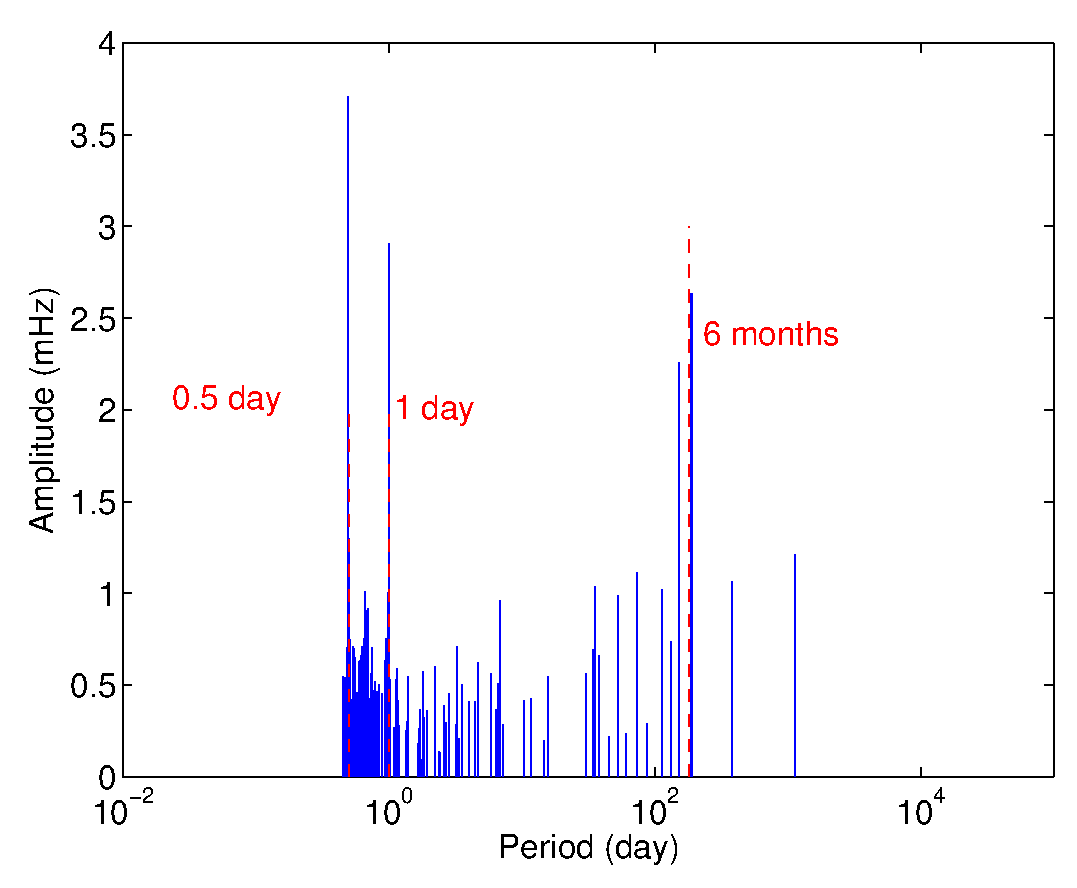
\includegraphics[width=\linewidth]{images/SparSpec_begining}
	\label{fig:SparSpec_pre}
  \caption{SparSpec Analyse der Abweichungen nach einem Fit mit konstanter Anomalie, ohne variable Terme.}
\end{minipage}
\hfill
\begin{minipage}[t]{.48\linewidth}
	\centering
	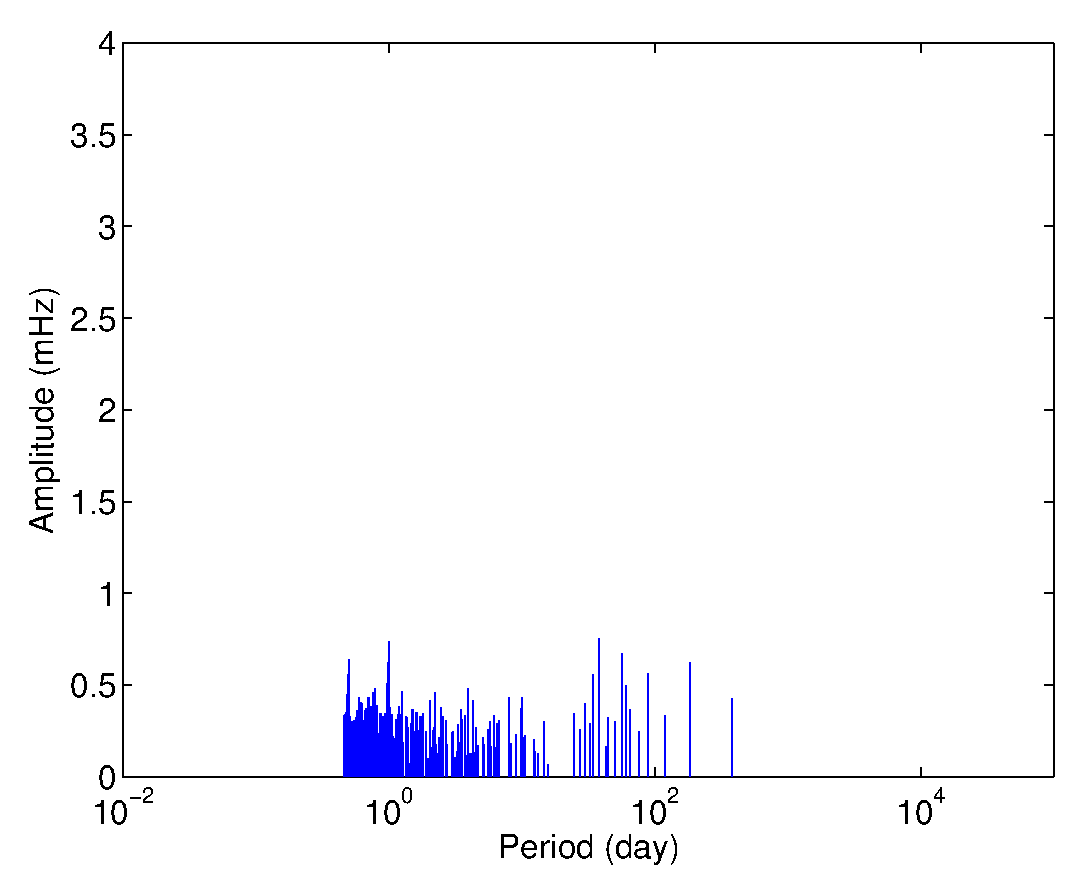
\includegraphics[width=\linewidth]{images/SparSpec_end}
	\label{fig:SparSpec_post}
  \caption{... und mit variablen Termen.}
\end{minipage}
 \end{figure}

Um die Existenz von periodischen Signalanteilen zu verdeutlichen, tragen die Abweichungen der Messwerte nach Entfernen der konstanten Anomalie im Frequenzbereich auf. Gewöhnlicherweise verwendet man dafür eine Fouriertransformation, da die Messpunkte im Falle der Pioneer-Daten allerdings nicht gleichmäßig verteilt sind, ist dies hier nicht möglich. Statt dessen verwendet man eine Software namens SparSpec.
Die periodischen Anteile des Signals lassen sich auf der daraus erhaltenen Abbildung \ref{fig:SparSpec_pre} sehr gut als herausragende Spitzen erkennen.
Die drei großen Peaks liegen bei $f_1=0.9974\pm0.004\ Tagen$, $f_2=\frac12(0.9972\pm0.004)\ Tagen$ und 
$f_3=189\pm32\ Tagen$, wobei $ 1\ Tag = 60 \cdot 60 \cdot 24 \:s = 86400\:s$ ist.
Bedenkt man das 1.0 siderischer Tag = 0.9972 Tage ist, so entspricht dies genau halbtägigen, täglichen und halbjährlichen Schwankungen.

Die Ursache für diese periodischen Terme dürfte nach gängiger Ansicht nicht in den Sonden zu suchen sein. Fehler im atmosphärischen Modell wären eine naheliegende Ursache für tägliche Variationen. Da diese jedoch von den Konditionen bei den Einrichtungen des DSN abhängen, müssten sie mit der Periode des Sonnentags und nicht des siderischen Tages verlaufen\cite{Levy2009}.
Anderson et al. ziehen für die Variationen Modellierungsfehler – wie Fehler in den Ephemeriden oder der Ausrichtung der Drehachse der Erde, oder fehlerhafte oder zu ungenaue Koordinaten der Messstationen – in Betracht\cite{Levy2009}\cite{Dittus2006}. % originalquelle?
Die Gruppe um Levey (GAP) hält dies jedoch für unwahrscheinlich, da diese Daten durch andere Beobachtungsmethoden
stark gestützt werden und es somit schwer wäre sie stark genug zu verändern um die gemessenen Effekte zu erklären. %Markward: Position offen geht auch

Sie nehmen in ihrer Untersuchung an, dass durch eine beliebige Ursache die Ausbreitung des Tracking-Signals auf
dem Weg zwischen Raumsonde und Erde verändert wird. Sie beschreiben die Ursache als Funktion des Winkels $\varphi$. Dieser wird definiert als die Differenz zwischen dem Azimutalwinkel der Antenne des DSN $\varphi_A$ und dem Azimutalwinkel der Pioneer-Sonde $\varphi_P$: $\varphi=\varphi_A-\varphi_P$. % siehe Grafik
Dieses Modell berücksichtigt also sowohl die Bewegung der Erde um die Sonne, als auch die Rotation der Erde um ihre Achse.
Die Beeinflussung des Signals wird nun mit Fourierkoeffizienten ($\upsilon_n$ und $\upsilon'_n$), beschrieben:
\begin{equation}
\Delta f = \sum_n (\upsilon_n(cos(n\varphi_u)+cos(n\varphi_d))+\upsilon'_n(sin(n\varphi_u)+sin(n\varphi_d))
\end{equation}
wobei $\varphi_u$ und $\varphi_d$ die Winkel $\varphi$ bei Up- beziehungsweise Down-link sind.
Nun können wir die die Fourierkoeffizienten sowie die konstante Anomalie an die Messwerte fitten. Wir verwenden dabei n = 1 und 2, das Hinzufügen von höheren Ordnungen bringt keine nennenswerte Verbesserung.

Dieses geometrische Modell beschreibt sowohl die täglichen als auch die jährlichen
Schwankungen und verringert die Standardabweichung der Messwerten von 9.8 mHz auf 5.5 mHz.
Auch die Spektralanalyse (Abb. \ref{fig:SparSpec_post}) dieses Fits zeigt die Verbesserung deutlich\cite{Levy2008}. % Besser zitieren
%mehr, weiter, ...

% Wie hängt das folgende mit dem obigen zusammen:
Nieto und Anderson weisen in \cite{Nieto2005} des weiteren darauf hin, das sich die jährliche zeitliche Änderung der Anomalie %von wann
grob durch eine Sinuswelle beschreiben lässt. Im Falle von Pioneer 10 hat diese eine Amplitude von $(0.525\pm0.155)\cdot10^{-8}cm/s^{-2}$ und im Fall von Pioneer 11 $(0.498\pm0.176)\cdot10^{-8}cms^{-2}$. Der Phasenunterschied der beiden Wellen beträgt 173.2°, was in etwa dem Winkelunterschied zwischen den ekliptikalen Längen\footnote{Ekliptikale Länge/Breite sind die zwei Himmelskoordinaten des ekliptikalen Koordinatensystems, welche die Ekliptik als Referenz zur Angabe der Position eines Objekts am Himmel verwendet.} der Flugrichtungen der Raumsonden entspricht, während die Amplituden etwa proportional zum Cosinus der ekliptikalen Breiten sind.

%Wohin damit:
Für die Betrachtung der veränderlichen Anteile der Anomalie muss die Kompressionszeit der Daten natürlich immer entsprechend kurz sein\cite{Nieto2005}.

\bigskip

\section{Klassische Erkl\"arungen}\label{klassisch}

Bevor man neue Theorien aufstellt um diese ungew\"ohnliche
Beschleunigung zu erkl\"aren, sollte man sich zun\"achst die
klassischen Erkl\"arungen ansehen, die die Beschleunigung erkl\"aren
k\"onnten bzw. eine Fehlerabsch\"atzung der Beschleunigung geben
k\"onnen. Hierzu teilte Anderson et al. \cite{Anderson2002} die Daten von Pioneer 10 in drei Intervalle
ein, die man durch den steigenden Abstand zur Sonne und Einfl\"usse von
anderen Himmelsk\"orpern abgrenzen muss. (Abb. \ref{fig:intervalle})

\begin{figure}[htbn]
\begin{center}
\noindent    
\psfig{figure=images/intervalle,width=0.8\linewidth,height=\textheight,keepaspectratio}
\end{center}
\vskip -10pt
  \caption{Abgrenzung der drei Datenintervalle von Pioneer 10 \cite{Anderson2002}}
\label{fig:intervalle}
\end{figure} 

\subsection{Externe Fehlerquellen}\label{extern}

\subsubsection{Strahlungsdruck der Sonne}

Durch den Impuls den die Photonen des Sonnenlichts auf die Fl\"ache der Sonde
\"ubertragen entsteht eine Kraft und damit letztlich auch eine
Beschleunigung. Diese ist zwar in Flugrichtung gerichtet, muss aber
f\"ur eine Fehlerrechnung und einer genauen zuerst betrachtet werden. Ein Modell f\"ur
den Strahlungsdrucks gab es schon vor Pioneer 10 und 11. Dieses Modell
formuliert eine Beschleunigung in Abh\"angigkeit der Ausrichtung und
Entfernung der Sonde zur Sonne.

\begin{equation}\label{eins}
a_{\mathit{sd}}(r)=-\frac{\kappa f_{s}A\cos \theta
(r)}{cMr^{2}}
\end{equation}

Dabei sind:
\begin{itemize}
\item $\mathit{f_s}=1367W/(\mathit{m\cdot AU})^2$
\item $A=r^2\pi =(1,37m)^2\pi $ (als sonnenzugewandte Oberfl\"ache der Sonde wird vereinfacht
die Fl\"ache der Parabolantenne verwendet)
\item $\theta $ ist der Winkel unter dem die Photonen auf $A$ treffen. Da der Winkel immer unter 1.5° ist wird er zu $\theta = 0\degree$ vereinfacht, was lediglich zu einem Verlust an Genauigkeit von $< 4 \cdot 10^{-12} \frac{cm}{s^2}$\cite{Markwardt2002} führt.
\item $c$ ist die Lichtgeschwindigkeit
\item $M$ ist die nominelle Masse der Sonde, zum Zeitpunkt an welchem die H\"alfte des
Treibstoffs verbraucht war (F\"ur Pioneer 10 wurden 241 kg angenommen)
\item $r$ ist der Abstand Sonde-Sonne in AU
\item $\kappa $ ist der effektive Absorptions/Reflexions-Koeffizient. F\"ur
Pioneer 10 wurde ein $\kappa_0=1,71 $ ermittelt\cite{Anderson2002}.
\end{itemize}

\bigskip

So erh\"alt man bei einem Abstand von 5,2 AU eine Beschleunigung von
$-(70,0\pm 3,5)\cdot 10^{-8}\mathit{cm}/s^{2}$ mit $\kappa_{5,2 AU}=1,77$.
Da der Strahlungsdruck wie alle anderen
Gesetze im 3-dimensionalen Raum dem $1/r^{2}$ Gesetzt folgt, war die
Beschleunigung bei 10 AU noch $-18,9\cdot 10^{-8}\mathit{cm}/s^{2}$
und bei 70 AU nur noch $-0,39\cdot 10^{-8}\mathit{cm}/s^{2}$. Da der
Strahlungsdruck der Sonne sehr genau von den Auswertungsprogrammen
modelliert werden kann, liegt der Fehler f\"ur Pioneer 10 zwischen 40
und 70 AU bei $0,001\cdot 10^{-8}\mathit{cm}/s^{2}$ und f\"ur Pioneer
11 zwischen 22 und 32 AU bei $0,006\cdot 10^{-8}\mathit{cm}/s^{2}$

Da die Masse durch die Verbrennung von Treibstoff mit der Zeit auch
ver\"anderte, erh\"alt man f\"ur die Ver\"anderung von $a_{p}$ f\"ur
die 3 Intervalle\cite{Anderson2002}:

\begin{equation}
\mathit{\delta a}_{p}=[(0,040\pm 0,035),(0,029\pm 0,025),(0,020\pm
0,017)]\cdot 10^{-8}\mathit{cm}/s^{2}
\end{equation}
Man bildet das gewichtete Mittel und erh\"alt f\"ur

\begin{equation}
a_{\mathit{sd}}=(0,03\pm 0,01)\cdot 10^{-8}\mathit{cm}/s^{2}
\end{equation}

Wenn man nun f\"ur Pioneer 11 das gleiche durchf\"uhrt erh\"alt man
\begin{equation}
a_{\mathit{sd}}=(0,09\pm 0,21)\cdot 10^{-8}\mathit{cm}/s^{2}
\end{equation}

Dies kann nicht die Anomalie erkl\"aren. Ist jedoch f\"ur die
Fehlerrechnung interessant.


\bigskip

\subsubsection{Der Sonnenwind}

Der Sonnenwind beschleunigt die Pioneers \"ahnlich wie Gl. \ref{eins}, nur das
man $\frac{f_{s}}{c}$ \ durch $m_{p}v^{2}n$ ersetzt. Hier ist
$n{\approx}5/\mathit{cm}^{3}$ die Protonendichte bei 1 AU und
$v{\approx}400\mathit{km}/s$ die Windgeschwindigkeit. So erh\"alt
man\cite{Anderson2002}:
\begin{equation}
a_{\mathit{sw}}(r)=-\frac{\kappa _{\mathit{sw}}m_{p}v^{2}nA\cos \theta
}{Mr^{2}}\approx -1,11\cdot
10^{-11}(20\frac{\mathit{AU}}{r})^{2}\mathit{cm}/s^{2}
\end{equation}

Da die Protonendichte um 100\% schwanken kann, ist die tats\"achliche
Beschleunigung unvorhersehbar. Unter der konservativen
Annahme, dass diese Beschleunigung um zwei Gr\"o{\ss}enordnungen
kleiner ist als die des Strahlungsdrucks, ist sie zu vernachl\"assigenden.


\bigskip

\subsubsection{Die Effekte der Sonnencorona}

Wie in Abschnitt 3.1.2 gesehen, ist der Effekt des Sonnenwindes auf die
Beschleunigung der Sonden vernachl\"assigbar. Jedoch muss man den
Einfluss der Sonnencorona auf die Radiosignale ber\"ucksichtigen. Denn
die Elektronendichte und der Gradient der Elektronendichte beeinflussen
die Ausbreitung von Radiowellen in einem Medium. Die Zeitverz\"ogerung einer S-Band Welle auf einem Weg $l$ l\"asst sich beschreiben als
\begin{equation}
\Delta t=\frac{\pm 1}{2\mathit{cn}_{\mathit{krit}}(\nu )}\int
_{\mathit{Sonnenmittelpunkt}}^{\mathit{Sonnencorona}}n_{e}(t,r)\mathit{dl}
\end{equation}
\cite{Anderson2002}

Mit
\begin{itemize}
\item $n_{\mathit{krit}}(\nu )=1,240\cdot 10^{4}(\frac{\nu
}{1}\mathit{MHz})^{2}\frac{1}{\mathit{cm}^{3}}$ ist die kritische
Plasmadichte f\"ur eine Tr\"agerfrequenz $\nu $

\item $n_{e}(t,r)$ ist die freie Elektronendichte im Sonnenplasma
\item Das positive Vorzeichen ist f\"ur Laufzeitdaten und das negative
f\"ur Dopplerdaten
\end{itemize}

Um den Einfluss der Sonnencorona auf die Radiowellen der
Pioneer-Sonden zu verstehen, kann die Elektronendichte der Corona als
Summe einer statischen und einer ver\"anderlichen Elektronendichte
modelliert werden. Da der ver\"anderliche Teil \ kaum Einfluss auf
Dopplerdaten hat\cite{Anderson2002}, reicht es ein statisches Modell der Sonnencorona
zu betrachten. F\"ur dieses Modell erh\"alt man eine freie
Elektronendichte von\cite{Anderson2002}:

\begin{equation}
n_{e}(r,t)=A(\frac{R_{s}}{r})^{2}+B(\frac{R_{s}}{r})^{2,7}\cdot
e^{-[\frac{\Phi }{\Phi _{0}}]^{2}}+C(\frac{R_{s}}{r})^{6}
\end{equation}
Aus den Daten der Cassini-Mission wurden f\"ur die Parameter A,B und C die
folgenden Werte ermittelt:

\begin{equation*}
A=6,0\cdot 10^{3}m
\end{equation*}
\begin{equation*}
B=2,0\cdot 10^{4}m
\end{equation*}
\begin{equation*}
C=0,6\cdot 10^{6}m
\end{equation*}
Dies nennt man das {\quotedblbase}Cassini Corona Model``. Die
Auswertungsprogramme ODP/Sigma und CHASMP haben f\"ur den Fehler der Beschleunigung aufgrund der Sonnencorona den
Wert

\begin{equation}
\sigma _{\mathit{corona}}=\pm 0,02\cdot
10^{-8}\mathit{cm}/s^{2}
\end{equation}
berechnet\cite{Anderson2002}.


\bigskip

\subsubsection{Lorentzkr\"afte}

Es ist nicht unwahrscheinlich dass die Sonden eine Ladung tragen, die im
elektromagnetischen Feld des Sonnensystems einen Einfluss auf die
Geschwindigkeit hat. Die magnetische Feldst\"arke im \"au{\ss}eren
Sonnensystem liegt bei unter $10^{-5}\mathit{Gauss}$\cite{Anderson2002}.
Unter der Annahme dass die Sonden eine maximale Ladung von $0,1-1,8\mu
C$\footnote{ %% ### Fussnote nicht mehr auf zwei Seiten splitten
Ich gebe hier deshalb einen Bereich an, da die Angaben in \cite{Null1976} auf der Tatsache beruhen, dass
Pioneer 10 bei Jupiter eine magnetische Feldst\"arke von 1,135 Gau{\ss}
gemessen h\"atte. Dies ist aber laut \cite{Anderson2002}, S. 29 falsch, da f\"ur Pioneer 10 nur eine
magnetische Feldst\"arke von 0,185 Gau{\ss} gemessen wurde (Pioneer 11
ma{\ss} durch ihre gr\"o{\ss}ere Ann\"aherung 1,135 Gau{\ss}).
\begin{equation*}
B=\frac{F_{B}}{\mathit{qv}}\ \ \mathit{mit}\ \ F=m\cdot
a\ \ \mathit{ergibt}\mathit{sich}\mathit{f\text{\"u}r}\mathit{die}\mathit{Ladung}\ \ q=\frac{\mathit{ma}}{\mathit{BV}}
\end{equation*}
mit \cite{Anderson2002}, S. 29:
\begin{equation*}
\begin{gathered}v=14,36\cdot 10^{3}m/s;\ B=0,185\cdot
10^{-4}T;\ m=241\mathit{kg};\ a=20\cdot 10^{-10}m/s^{2}\end{gathered}
\end{equation*}
ergibt sich:
\begin{equation*}
q=1,8143\mu C
\end{equation*}}
tragen k\"onnen errechnet sich eine Beschleunigung von
\begin{equation}
a=\frac{\mathit{Bqv}}{M}=\frac{1\cdot 10^{-9}T\cdot 1\cdot
10^{-6}C\cdot 14,36\cdot 10^{3}m/s}{251,883\mathit{kg}}=5,7\cdot
10^{-14}m/s^{2}
\end{equation}
Mit 
\begin{itemize}
\item $B$ ist die magnetische Flussdichte
\item $q$ ist die Ladung der Sonde
\item $v$ ist die Geschwindikeit der Sonde
\end{itemize}

Diese Beschleunigung kann man vollst\"andig vernachl\"assigen.


\bigskip

\subsubsection{Die Gravitation des Kuiperg\"urtel}

Unter der Annahme, dass sich im Kuiperg\"urtel etwa 1 Erdmasse an
Partikeln befinden hat man 3 Staubverteilungen gepr\"uft: 1) eine
gleichm\"a{\ss}ige Verteilung, 2) eine 2:1 Resonanz Verteilung \ mit
einem Maximum bei 47,8 AU und 3) eine 3:2 Resonanz Verteilung mit einem
Peak bei 39,4 AU. Die letzten 2 Verteilungen wurden deswegen
ausgew\"ahlt, da diese Verh\"altnisse bei dem Resonanzeffekt von Neptun
auf Pluto beobachtet wurden. Abb.\ref{fig:kuiper} zeigt die Beschleunigung auf
Pioneer 10 von 30 bis 65 AU. Hier erkennt man eine Beschleunigung in der
Gr\"o{\ss}enordnung von $10^{-9}\mathit{cm}/s^{2}$. \ In Abb.\ref{fig:kuiper}
erkennt man zus\"atzlich, dass die Beschleunigung nicht konstant ist.
Da der Wert zwei Gr\"o{\ss}enordnungen unter der Anomalie liegt und
nicht konstant ist, kann man den Kuiperg\"urtel als Ursache der
Anomalie ausschlie{\ss}en. Infrarotmessungen von 2002 haben eine Masse
von ca. 0,3 Erdmassen im Kuiperg\"urtel entdeckt. Dies wird in der
Fehlerrechnung mit \ $\sigma _{\mathit{KG}}=\pm 3\cdot
10^{-10}\mathit{cm}/s^{2}$ ber\"ucksichtigt\cite{Anderson2002}.


\begin{figure}[htbn]
\begin{center}
\noindent    
\psfig{figure=images/kuiper,width=0.5\linewidth,height=\textheight,keepaspectratio}
\end{center}
\vskip -10pt
  \caption{Mögliche Beschleunigung der Pioneer-Sonden durch die Gravitation des Kuipergürtels \cite{Anderson2002}}
\label{fig:kuiper}
\end{figure} 


\bigskip

\subsection{Sondeninterne Fehlerquellen}\label{intern}

\subsubsection{Radiowellenr\"ucksto{\ss}}

Die Pioneer-Sonden haben eine Sendeleistung von 8 W, die wie folgt
abgestrahlt wird:
\begin{equation}
P_{\mathit{SL}}=\int _{0}^{\theta _{\mathit{max}}}\sin \theta \rho
(\theta )d\theta
\end{equation}
Dabei ist $\rho (\theta )$ die Leistungsverteilung.

Die Beschleunigung der Sonde durch die Radiowellen l\"asst sich
berechnen mit:
\begin{equation}
b_{\mathit{SL}}=\frac{\beta P_{\mathit{SL}}}{\mathit{Mc}}
\end{equation}
wobei $b_{\mathit{SL}}$ von der Erde weg zeigt. Dabei ist $\beta $ die
partielle Komponente des Strahlungsmoments, welche in entgegengesetzter
Richtung zu $a_{p}$ zeigt\cite{Anderson2002}:
\begin{equation}
\beta =\frac{1}{P_{\mathit{SL}}}\int _{0}^{\theta _{\mathit{max}}}\sin
\theta \cos \theta \rho (\theta )d\theta
\end{equation}
Messungen  zeigten\cite{Anderson2002}, dass man den Strahl als konisch annehmen kann.
Mit einem Gesamt\"offnungs\-winkel von $\theta =3,75{}^{\circ}$ ist
$\beta =0,99\pm 0,01$ und damit $w_{\mathit{SL}}=1,10\cdot
10^{-8}\mathit{cm}/s^{2}$.

Mit einem Fehler der Sendeleistung und der Ungenauigkeit der Masse
erh\"alt man als Ergebnis f\"ur die Beschleunigung der Sonden durch die
Sendeleistung
\begin{equation}
a_{\mathit{SL}}=-1,10\pm 0,11\cdot 10^{-8}\mathit{cm}/s^{2}
\end{equation}


\newpage 

\subsubsection{Ungleichm\"a{\ss}ige Abstrahlung der RTGs}

W\"ahrend dem Flug zum Jupiter war die Sonde relativ nahe an der Sonne.
Eine Erkl\"arung f\"ur die Beschleunigung k\"onnte nun folgende sein:
Die Fl\"achen der RTGs\footnote{RTG steht für radioisotope thermoelectric generator, zu Deutsch Radionuklidbatterie und ist im äußeren Planetensystem die einzig sinnvolle Energiequelle. Die Energieversorgung einer Raumsonde durch Solarzellen ist nicht praktikabel, da die Solarzellen enorme Flächen bräuchten um genug Leistung bereit zu stellen. In einem RTG zerfällt auf natürliche Weise ein $\alpha$-Strahler und erzeugt durch den Stoss der ausgesendeten Heliumkerne an anderen Atomen Wärme. Diese W\"arme nehmen thermoeletrische Bauelemente auf und wandeln sie direkt in elektrische Energie um.}, die der Sonne zugewandt waren, haben eine
h\"ohere Strahlendosis durch den Sonnenwind erfahren als die der Sonne
abgewandten. Dies geschah gleichzeitig mit dem Auftreffen von interplanetarem Staub auf die sonnenabgewandten Seiten. Dadurch entstand ein
Strahlungsgradient und somit eine ungleichm\"a{\ss}ige Abstrahlung der
RTGs. Durch die spezielle Bauweise der K\"uhlrippen aus einer
Magnesiumlegierung, die mit einem Zirkonium-Natrium Silicat beschichtet
war, besitzen die K\"uhlrippen einen hohen Emissionskoeffizienten
von ca. 0,9 und einen geringen Absorptionskoeffizienten von ca. 0,2. Um
nun $a_{p}$ hervorzurufen m\"usste es eine unterschiedliche
Abstrahlung in Front/Heck- Ausrichtung von 10\% gegeben haben. Nach
unserem Kenntnisstand des Sonnenwindes und des interplanetaren Staubs
ist es nicht m\"oglich, dass diese zwei Ph\"anomene einen derart
gro{\ss}en Gradienten mit dem richtigen Vorzeichen erzeugen k\"onnen.
Dies wurde durch visuelle Beweise der Voyager Sonden gest\"utzt\cite{Anderson2002}.

W\"ahrend den Flyby Man\"overn wurden die Sonden jedoch sehr hoher
Strahlung ausgesetzt, die eine Besch\"adigung der RTGs zur Folge haben
k\"onnte. Man h\"atte also w\"ahrend eines Flyby Man\"overs einen
Anstieg in der thermischen Emission beobachten m\"ussen. Da f\"ur die
Oberfl\"achenenergiebelastung $F\alpha T^{4}$ gilt, h\"atte man eine
Temperaturdifferenz an den K\"uhlrippen beobachten m\"ussen. Die
Durchschnittstemperatur der K\"uhlrippen lag bei ca. 440 K \cite{Anderson2002}. Um
$a_{p}$ zu erkl\"aren m\"usste ein Unterschied von 10\% bzw. $\approx$12,2 K
herrschen. Dieser Unterschied wurde jedoch nicht beobachtet und somit
kann auch dies als Ursache f\"ur die Anomalie ausgeschlossen werden. Um
diesem Effekt dennoch gerecht zu werden, wird f\"ur die Fehlerrechnung
eine unterschiedliche Abstrahlung von 1\% angenommen. Bei einer
thermischen Leistung von 2000 W liegt eine unterschiedliche Abstrahlung
von 10 W in Front/Heck-Ausrichtung vor. Da die K\"uhlrippen in einem
Abstand von 30{\textdegree} angebracht sind, ergibt sich aus
$[10W]\cdot \int _{0}^{\pi }[\sin \Phi ]d\Phi /\pi \approx
6,12W$\cite{Anderson2002} (da 4 der 12 Rippen senkrecht und parallel zur Flugrichtung
stehen) eine Ungenauigkeit von

\begin{equation}
\sigma _{\mathit{UA}}=0,85\cdot 10^{-8}\mathit{cm}/s^{2}
\end{equation}


\bigskip

\subsubsection{Aussto{\ss} von Helium aus den RTGs}

Eine weitere Erkl\"arung der anomalen Beschleunigung ist, dass durch den
$\alpha ${}-Zerfall von Pu-238 Helium aus den RTGs austritt. Die RTGs
der Pioneer Sonden wurden so konstruiert, dass das Helium aus der
Hitzequelle in den thermoelektrischen Konverter diffundieren kann. Der
Konverter ist mit einem Dichtungsring(O-Ring) abgeschlossen, der es dem Helium
allerdings erm\"oglicht in den Weltraum zu entweichen. Im gesamten Brennstoff
 der RTGs sind 5,8 kg Pu-238 enthalten\cite{Anderson2002}. Mit einer
Halbwertszeit von 87,74 Jahren werden pro Jahr ca. 0,77 g Helium mit einer
Temperatur von 433 K ausgesto{\ss}en. Dies entspricht nach $E_kin=3/2 kT$ einer
Geschwindigkeit von 1,22 km/s. Mit der Raketengleichung
\begin{equation}
a(t)=-v(t)\frac{d}{\mathit{dt}}[\ln M(t)]\ ,
\end{equation}
unser nominellen Pioneer 10 Masse von 241 kg und der Annahme, dass das
Helium die RTGs ungerichtet verl\"asst, erh\"alt man eine
Beschleunigung von $1,16\cdot 10^{-8}\mathit{cm}/s^{2}$.

Der Gasaustoss ist jedoch nicht ungerichtet, sondern, da der O-Ring an
der Seite der RTGs angebracht ist, in Richtung Sonne. Durch die
K\"uhlrippen der RTGs wird au{\ss}erdem noch Helium elastisch
reflektiert, sodass man auf eine Beschleunigung aufgrund des
Heliumaussto{\ss}es von
\begin{equation}
a_{\mathit{He}}=-(0,15\pm 0,16)\cdot 10^{-8}\mathit{cm}/s^{2}
\end{equation}
kommt\cite{Anderson2002}.


\bigskip

\subsubsection{Gasleck im Antriebssystem}

Da es keine perfekten Ventile gibt, muss man immer mit einem leichten
Gasaustritt im Antriebssystem rechnen. Einige Sonden\cite{Anderson2002} haben
deswegen Beschleunigungen von bis zu $10^{-7}\mathit{cm}/s^{2}$
erfahren. Das Antriebssystem der Pioneers besteht aus drei Paar
Korrekturd\"usen, die im 120{\textdegree} Abstand um die Parabolantenne
angebracht sind. Von diesen drei Paaren sind zwei parallel zur
Sonnenl\"angsachse ausgerichtet um die Pr\"azession der Parabolantenne
zu steuern. Ein Paar ist tangentiell zur Antenne positioniert um die
Rotation zu steuern. Aus den Ver\"anderungen der Rotationsrate in den
Intervallen i=I,II,III ist die Kraft eines Gaslecks mit einem Hebelarm
von R=1,37 m und einem Tr\"agheitsmoment von
$I_{z}=588,3\mathit{kg}\cdot\ m^{2}$
\begin{equation}
F_{\theta }=\frac{I_{z}\theta }{R}=(2,57;12,24;1,03)\cdot
10^{2}N
\end{equation}

Um nun die Kraft der zwei anderen Korrekturd\"usen abzusch\"atzen, nimmt
man an, dass diese das gleiche Gasleck haben, wie die
Rotationskorrekturd\"usen. So kann man nun annehmen\cite{Anderson2002}, dass
\begin{equation}
F_{\mathit{GL}}\simeq \pm \sqrt{(2)}F_{\theta }=(\pm 3,64;\pm
17,31;\pm 1,46)\cdot 10^{2}N
\end{equation}
ist. Unter der weiteren Annahme dass die Fehler normalverteilt sind,
liegt der Fehler f\"ur Pioneer 10 bei
\begin{equation}
\sigma _{\mathit{GL}}=\pm 0,56\cdot 10^{-8}\mathit{cm}/s^{2}
\end{equation}
Dies ist die gr\"o{\ss}te Ungenauigkeit, aber jedoch nicht gro{\ss}
genug um die Pioneer-Anomalie zu erkl\"aren.


\bigskip

\subsubsection{R\"ucksto{\ss} durch thermische Abstrahlung}\label{Hitze}

In der urspr\"unglichen Arbeit von 2002 \cite{Anderson2002} standen den Autoren nur
begrenzte Telemetriedaten zur Verf\"ugung. So haben sie einen Wert
f\"ur den R\"ucksto{\ss} der thermischen Abstrahlung und der
ungleichm\"a{\ss}igen Abk\"uhlung der Sonden von
$a_{\mathit{tA}/\mathit{Ak}}=0,55\pm 0,73\cdot
10^{-8}\mathit{cm}/s^{2}$ errechnet \cite{Anderson2002}[Tabelle X]. 2003 wurde jedoch
eine Arbeit ver\"offentlicht, die eine gerichtete thermische
Abstrahlungsleistung von 52 W angab. Dieser hohe Wert wurde durch
andere Berechnungen, wie die Annahme eines Lambertstrahlers(ca. 45 W)
oder eine Finite Elemente Methode(ca. 48 W), gest\"utzt\cite{Turyshev2010}. Diese Berechnungen zeigen, dass die Kraft der
thermischen Strahlung vollkommen untersch\"atzt wurde. Leider waren
auch die neuen Werte nur auf groben Absch\"atzungen der thermischen und
elektrischen Leistung an Board der Sonden gest\"utzt. Au{\ss}erdem
machen sie keine Aussagen \"uber den zeitlichen Verlauf der
Abstrahlung. Da f\"ur beide Pioneer Missionen mittlerweile alle
Telemetriedaten vorliegen wurden neue Untersuchungen der thermischen
Abstrahlung der Sonden durchgef\"uhrt.

Hier wurden zwei Hauptthermalquellen ausgemacht: Zum einen die RTGs und
zum anderen die elektrischen Ger\"ate an Board.


\bigskip
Da sich alle 4 RTGs einer jeden Pioneer Sonde zeitlich gleich verhalten,
kann man sie als eine Hitzequelle beschreiben. Die Leistung der RTGs
verh\"alt sich nach dem Zerfallsgesetz mit
\begin{equation}
P_{\mathit{rtg}}(t)=2^{\frac{-(t-t_{0})}{T}}P_{\mathit{rtg}}(t_{0})
\end{equation}
mit dem Zeitpunkt $t_0$ an dem die
Leistung $P_{\mathit{rtg}}(t_{0})=(650\pm 1)W/\mathit{RTG}$ gemessen
wurde und der Halbwertszeit von Pu-238 von T=87,74 a. Da man f\"ur die
abgenommene elektrische Leistung die genauen Daten kennt (Abb.\ref{fig:hitze}),
l\"asst sich die W\"armeleistung schreiben als
\begin{equation}
B_{\mathit{rtg}}(t)=P_{\mathit{rtg}}(t)-P_{\mathit{el}}(t)
\end{equation}


\bigskip

\begin{figure}[htbn]
\begin{center}
\noindent    
\psfig{figure=images/hitze,width=0.8\linewidth,height=\textheight,keepaspectratio}
\end{center}
\vskip -10pt
  \caption{Hitzeentwicklung der RTGs (rote Datenpunkte, Skala auf der linken Seite) und der elektronischen Geräte (grüne Datenpunkte, Skala auf der rechten Seite) über die Funktionsdauer von Pioneer 10 \cite{Turyshev2010}}
\label{fig:hitze}
\end{figure} 


\bigskip

In Abb. \ref{fig:hitze} ist au{\ss}erdem noch die elektrische Leistung aufgetragen,
die von ca. 160 W am Start der Mission langsam auf ca. 60 W abfiel, als
Pioneer 10 das letzte Signal sendete. Teilweise wurde die entnommene
elektrische Leistung aus den RTGs in den Ger\"aten unterschiedlich stark in Hitze umgewandelt
und abgestrahlt. Obwohl die Verteilung der Hitzequellen innerhalb der
Sonde nicht gleichm\"a{\ss}ig war, blieb die Temperaturverteilung in
der Sonde als Funktion der Zeit linear\cite{Turyshev2010}. Somit kann
man die Hitzeabstrahlung aufgrund von elektrischen Ger\"aten als eine
Hitzequelle behandeln. Die Daten hierf\"ur liefert die Telemetrie(Abb.\ref{fig:hitze}).

Die Berechnung der Kraft auf die Sonden gestaltet sich etwas einfacher,
da durch die Spinstabilisierung die Kraft \textit{F }nur entlang des
Einheitsvektors der Rotationsachse \textit{\bf s} berechnet werden muss:
\begin{equation}
F=\frac{1}{c}(\xi _{\mathit{rtg}}B_{\mathit{rtg}}+\xi
_{\mathit{el}}B_{\mathit{el}}){\bf s}
\end{equation}

Die Faktoren $\xi _{\mathit{rtg}}$ und $\xi _{\mathit{el}}$ lassen
sich aus der Geometrie und den thermischen Eigenschaften der Sonden
berechnen\cite{Turyshev2010}.

Die Berechnung dieser Kraft ist Bestandteil aktueller Studien zur
Pioneer-Anomalie. Auf jeden Fall belegen sie den vollkommen
untersch\"atzten Einfluss der thermischen Abstrahlung auf die
Beschleunigung. Mithilfe der neuen, kompletten Telemetriedaten ist es
nun m\"oglich sehr gute Finite Elemente Modelle der Pioneer Sonden im
Bezug auf die Hitzeverteilung zu erstellen. Sollte die Anomalie, wenn
auch nur teilweise, von dieser thermischen Kraft erkl\"art werden, muss
man sich erneut Gedanken \"uber die Konstanz von $a_{p}$ machen.


\bigskip

\subsection{Fehlertabelle und endg\"ultiges Ergebnis}

In Kapitel \ref{extern} und \ref{intern} haben wir gesehen, dass die meisten Effekte, die 
die Pioneer Sonden erfahren, nur zu einem sehr kleinen Teil Einfluss auf die
Beschleunigung haben. Wir haben in dieser Arbeit nur die wichtigsten
Fehlerquellen zusammengefasst. Diese und andere Fehlerquellen, ihre
Werte und Ungenauigkeiten sind in nachfolgender Tabelle aufgelistet.


\bigskip
\begin{table}[htbn]\label{fehler}
\newcommand{\mc}[3]{\multicolumn{#1}{#2}{#3}}
\centering
\begin{tabular}{|c|c|c|}
\hline
Beschreibung &
Wert $\cdot (10^{-8}) cm/s^2$ &
$\sigma\ in\ (10^{-8}) cm/s^2$\\ \hline
\mc{3}{|c|}{\bf 1. Externe Fehlerquellen} \\ \hline
Strahlungsdruck der Sonne &
\raggedleft -0,03 &
 0,01\\ \hline
Sonnenwind &
~
 &
 {\textless}10\^{}-3\\ \hline
Sonnencorona &
~
 &
 0,02\\ \hline
Elektromagnetische Lorentzkr\"afte &
~
 &
 {\textless}10\^{}-4\\ \hline
Einfluss der Gravitation des Kuiperg\"urtel &
~
 &
 0,03\\ \hline
Einfluss der Erdorientierung &
~
 &
 0,001\\ \hline
Mechanische und Phasenstabilit\"at der DSN Antennen &
~
 &
 {\textless}0,001\\ \hline
Phasenstabilit\"at und Uhren &
~
 &
 {\textless}0,001\\ \hline
DSN Antennen Orte &
~
 &
 {\textless}10\^{}-5\\ \hline
Troposph\"are und Ionosph\"are &
~
 &
 {\textless}0,001\\ \hline
~
 &
~
 &
~
\\ \hline
\mc{3}{|c|}{\bf 2. Sonden interne Fehlerquellen}\\ \hline
R\"ucksto{\ss} der Radiowellen &
\raggedleft -1,1 &
 0,11\\ \hline
Hitze, reflektiert von der Sonde &
\raggedleft {}0,55 &
 0,55\\ \hline
Ungleichm\"a{\ss}ige Hitzeabstrahlung der RTGs &
~
 &
 0,85\\ \hline
Ungleichm\"a{\ss}ige Abk\"uhlung der Sonden &
~
 &
 0,48\\ \hline
Heliumaussto{\ss} aus den RTGs &
\raggedleft -0,15 &
 0,16\\ \hline
Gaslecks &
~
 &
 0,56\\ \hline
Unterschiede zwischen den Sonden &
\raggedleft -0,17 &
 0,17\\ \hline
~
 &
~
 &
~
\\ \hline
\mc{3}{|c|}{\bf 3. Rechnerische Fehlerquellen}\\ \hline
Numerische Stabilit\"at der Finite Elemente Methode &
~
 &
 0,02\\ \hline
Genauigkeit der Fehlerabsch\"atzung und Modelle &
~
 &
 0,13\\ \hline
Mismodellierung von Man\"overn &
~
 &
 0,01\\ \hline
Mismodellierung der Sonnencorona &
~
 &
 0,02\\ \hline
Jahres- und Tagesschwankungen &
~
 &
 0,32\\ \hline
\end{tabular}
\caption{Fehlertabelle}
\label{tab:fehler}
\end{table}

\noindent Das Ergebnis der anormalen Beschleunigung von Pioneer 10 und 11 liegt
bei\cite{Anderson2002}
\begin{equation}
a_{p(\mathit{gemessen})}=(7,84\pm 0,01)\cdot
10^{-8}\mathit{cm}/s^{2}\ .
\end{equation}
Bezieht man nun die Werte der Fehler und deren Ungenauigkeit von Kapitel
\ref{extern} und \ref{intern} mit ein, so erh\"alt man mit den Werten der Fehlertabelle
und mit
\begin{equation}
a_{p}=a_{p(\mathit{gemessen})}-(w_{p}\pm \sigma _{p}) \ ,
\end{equation}
wobei $w_{p}$ der Wert und $\sigma _{p}$ die jeweilige Ungenauigkeit
ist, den bekannten Wert f\"ur $a_{p}=(8,74\pm 1,33)\cdot
10^{-8}m/s^{2}$.

\FloatBarrier

\section{ Dunkle Materie}

Nachdem die Pioneer-Anomalie entdeckt wurde, kamen erste Theorien auf,
dass die Anomalie ein Indiz f\"ur Dunkle Materie in unserem
Sonnensystem sein k\"onnte. Verschiedene Verteilungen der Dunklen
Materie wurden durchgerechnet und so kann zum Beispiel eine Scheibe mit
einer Dichte von etwa $4\cdot 10^{-16}\mathit{kg}/m^{3}$ im
\"au{\ss}eren Sonnensystem die Anomalie erkl\"aren. Allerdings d\"urfte
diese Dunkle Materie nicht wie leuchtende Materie gravitativ
Beeinflussbar ist\cite{Turyshev2010}. Sprich, dass diese Scheibe die nicht
von Planeten beeinflusst und somit angeh\"auft wird. Dies ist jedoch
unwahrscheinlich. Wenn die Pioneer-Anomalie einen gravitativen Ursprung
h\"atte, so m\"usste sie nach Newton mit  $1/r^{2}$ abnehmen. Eine
derartige Abnahme h\"atte man in den 2002 vorliegenden Datenintervallen
beobachten m\"ussen, was aber nicht geschehen ist. Ein weiteres
Argument gegen die Dunkle Materie als Grund f\"ur die Pioneer-Anomalie
ist die Masse und Dichte von Dunkler Materie, die n\"otig w\"aren um
den Effekt zu verursachen. Es w\"are in einem Abstand von 50 AU eine
Masse von mindestens  $3\cdot 10^{-4}$ Sonnenmassen (sprich 
$5,967\cdot 10^{26}\mathit{kg}$) mit einer Dichte von  $6,0\cdot
10^{18}\mathit{kg}/\mathit{AU}^{3}$ n\"otig. \cite{Xu2008} argumentiert jedoch, dass \"uber die gesamte Lebensdauer
von unserem Sonnensystem von 4,5 Ga sich maximal eine Dichte von 
$2,0\cdot 10^{17}\mathit{kg}/\mathit{AU}^{3}$ h\"atte ansammeln
k\"onnen. Au{\ss}erdem sei die Masse an Dunkler Materie im gesamten
Sonnensystem nur ca. {}10\textsuperscript{20 }kg, womit die
Pioneer-Anomalie in keiner Weise erkl\"art w\"are.


\section{Dunkle Energie}


\bigskip

Schon fr\"uh fiel auf, dass f\"ur den Wert der Pioneer-Anomalie
$a_{p}\simeq \mathit{cH}_{0}$ gilt, wenn c die
Vakuumlichtgeschwindigkeit und $H_0$ die
derzeitige Hubble-Konstante ist. Deshalb wurden Vermutungen
laut, dass die Anomalie mit der Ausdehnung des Universums und somit mit
der Dunklen Energie in Zusammenhang steht\cite{Turyshev2010}. Die Idee hierzu ist,
dass die Anomalie gar keine echte Beschleunigung ist, sondern nur das
Doppler-Signal durch die Ausdehnung des Universums beeinflusst wird.
Die Grundfrage hier war also ob die Dunkle Energie einen messbaren
Einfluss auf elektromagnetische Wellen hat.


\bigskip

Die Sonde bewegt sich mit der Geschwindigkeit v. Demnach w\"are
die Beschleunigung durch das sich ausdehnende Universum $a_H$:

\begin{equation*}
a_{H}=v\cdot H_{0}=\frac{v}{c}\cdot c\cdot H_{0}
\end{equation*}

Man sieht deutlich, dass die Beschleunigung
$a_H$ um den Faktor v/c kleiner w\"are,
als die beobachtete $a_p$
Au{\ss}erdem ist $c\cdot H_{0}$ f\"ur 
$H_{0}=73,2\frac{\mathit{km}}{s\cdot \mathit{Mpc}}$ nur eine
Ann\"aherung an den tats\"achlichen Wert der Anomalie. Um den exakten
Wert f\"ur $a_p$ zu erhalten br\"auchte
man eine Hubble-Konstante mit einem Wert von $H_{0}=95\pm
14\frac{\mathit{km}}{s\cdot \mathit{Mpc}}$. Ein weiteres
Argument gegen den Einfluss der Dunklen Energie ist, dass die
Beschleunigung in Richtung Sonne zeigt. W\"are die Dunkle Energie
tats\"achlich die Ursache, w\"urden die Pioneer-Sonden von der Sonne
bzw. der Erde weg beschleunigt. Im Doppler-Signal w\"urde sich das in
einer Rotverschiebung \"au{\ss}ern, statt in der beobachteten
Blauverschiebung.


\bigskip

\section{Modifizierte Newtonsche Mechanik (MOND)}


Die modifizierte newtonsche Mechanik (MOND) wurde Mitte der 1980-er
Jahre von Mordehai Milgrom als Gegenentwurf zur dunklen Materie
entwickelt. Ihre urspr\"ungliche Motivation ist es die gemessene
abflachende Rotationskurve von Galaxien zu erkl\"aren, die sich
deutlich von der Kurve unterscheidet, die nach den keplerschen
Gesetzten berechnet wurde. Das soll erreicht werden indem das zweite
newtonsche Gesetz bzw. das Gravitationsgesetz modifiziert wird. 


\bigskip


Das zweite newtonsche Axiom besagt, dass eine Masse m, an der eine Kraft
F anliegt, die Beschleunigung a erf\"ahrt: 

\begin{equation}
F=m\cdot a
\end{equation}

Dieser Zusammenhang kann allerdings f\"ur sehr kleine Beschleunigungen
nur sehr schwer bis gar nicht experimentell \"uberpr\"uft und
nachgewiesen werden. In Galaxien bewirkt die Schwerkraft der Sterne
aber nur solche kleinen Beschleunigungen, da sie sehr weit voneinander
entfernt sind. Milgroms Idee \cite{Bekenstein1984} war es daher das zweite newtonsche
Gesetz f\"ur sehr kleine Beschleunigungen abzuwandeln in

\begin{equation}
F=m\cdot a\cdot \mu (a/a_{0})
\end{equation}

 $a_{0}$ ist eine neue Naturkonstante, die angibt, ab welchen
Beschleunigungen die Modifikation wirksam wird. Milgrom bestimmte sie
aus den Messungen der Rotationsgeschwindigkeiten m\"oglichst vieler
Galaxien als ungef\"ahr

\begin{equation*}
a_{0}=2\cdot 10^{-8}\frac{\mathit{cm}}{s^{2}}
\end{equation*}
$\mu (x)$ ist eine unspezifizierte Funktion, welche folgende
Bedingungen erf\"ullt:

\begin{equation*}
\mu \left( x \right) \approx
\begin{cases}
1 \qquad \mathrm{wenn} \left| x \right| \ll 1 \\
x \qquad \mathrm{wenn} \left| x \right| \gg 1 
\end{cases}
\end{equation*}

In der Literatur sind die f\"ur  $\mu (x)$ am h\"aufigsten verwendeten
Funktionen:

\begin{equation*}
\mu (x)=\frac{x}{1+x}
\qquad
\mu (x)=\frac{x}{\sqrt{1+x^{2}}}
\end{equation*}

Will man jetzt MOND in Hinblick auf die Pioneer Anomalie \cite{Turyshev2010}
\"uberpr\"ufen, muss man als erstes betrachten, welche Auswirkungen die
Theorie auf die Zentripetalbeschleunigung  $a_{z}$ einer Masse m hat,
die sich im Gravitationsfeld eines K\"orpers der Masse M befindet.

Nach Newton gilt mit der Gravitationskonstante G:

\begin{equation}
F_{g}=\frac{G\cdot {M\cdot m}}{r^{2}}
\end{equation}

Damit gilt f\"ur  $a_{z}$

\begin{equation}
a_{z}=\frac{v^{2}}{r}=\frac{G\cdot {M}}{r^{2}}
\end{equation}

L\"ost man diese Gleichung nach  $v^{2}$ auf, so erh\"alt man:

\begin{equation}
v^{2}=\frac{G\cdot M}{r}
\end{equation}

Nach MOND gilt f\"ur sehr kleine Beschleunigungen:

\begin{equation}
a_{z}\mu (\frac{a_{z}}{a_{0}})=\frac{G\cdot {M}}{r^{2}}
\end{equation}

Da  $\frac{a_{z}}{a_{0}}\ll 1$ gilt  $\mu
(\frac{a_{z}}{a_{0}})=\frac{a_{z}}{a_{0}}$

Setzt man dies nun in die obige Gleichung ein und l\"ost nach  $a_{z}$
auf, so erh\"alt man:

\begin{equation}
a_{z}=\frac{\sqrt{M\cdot G\cdot a_{0}}}{r}
\end{equation}

Mit  $a_{z}=\frac{v^{2}}{r}$ erh\"alt man hier f\"ur  $v^{2}$

\begin{equation}
v^{2}=\sqrt{M\cdot G\cdot a_{0}}
\end{equation}

Zusammenfassend gilt also nach der modifizierten newtonschen Dynamik:

\begin{equation*}
v^{2}=
\begin{cases}
\qquad \frac{G\cdot M}{r} \qquad \quad \, \textrm{wenn } a_{z}\gg a_{0} \textrm{ oder kleine Abst\"ande} \\
\sqrt{M\cdot G\cdot a_{0}} \qquad \textrm{wenn } a_{z}\ll a_{0} \textrm{ oder gro{\ss}e Abst\"ande}
\end{cases}
\end{equation*}
Betrachtet man nun die Pioneer-Anomalie, kann man davon
ausgehen, dass $a_{0}\ll \frac{G\cdot M}{r}$. \\
W\"ahlt man nun $\mu (x)=1+\frac{\zeta }{x}$ bekommt
man f\"ur $a_{z}$ folgendes Ergebnis:

\begin{equation}
a_{z}=-\ \frac{G\cdot M}{r^{2}}-\zeta \cdot a_{0}
\end{equation}
F\"ur $\zeta =7$ ist 

\begin{equation*}
\zeta \cdot a_{0}=8,4\cdot 10^{-8}\frac{\mathit{cm}}{s^{2}}
\end{equation*}
was in etwa der anomalen Beschleunigung der Pioneer-Sonden entspricht.


\bigskip


Gundlach et al.\cite{Grundlach2007} nahmen die MOND-Theorie zum Anlass ,das zweite
newtonsche Gesetz f\"ur sehr kleine Beschleunigungen zu \"uberpr\"ufen.
Mit Hilfe eines Torsionspendels gelang es ihnen gute Messungen bis zu
einer Beschleunigung von  $5\cdot 10^{-12}\frac{\mathit{cm}}{s^{2}}$
durchzuf\"uhren. Dabei konnte keine Verletzung von Newtons Aussage
festgestellt werden. Dies stellt allerdings keinen direkten Widerspruch
zur MOND-Hypothese dar, da diese fordert, dass Messungen au{\ss}erhalb
des Einflussbereiches anderer gr\"o{\ss}erer Beschleunigungen
durchgef\"uhrt werden m\"ussen. Diese Bedingung ist auf der Erde durch
ihr Gravitationsfeld und dem des Sonnensystems nicht gegeben. Die
Ergebnisse zeigen jedoch, dass es nicht m\"oglich ist, MOND von
fundamentalen Prinzipien abzuleiten unter der Auflage, dass der
Formalismus  $F=m\cdot a$  unter Laborbedingungen reproduziert.


Nach der modifizierten newtonschen Dynamik m\"ussten auch die Planeten,
vor allem die \"au{\ss}eren, die selbe Anomalie aufweisen wie die
Pioneer Sonden. Die Planetenbahnen sind aber seit langem sehr genau
bekannt und weisen keine Abweichungen auf, die auf eine solche
Beschleunigung hinweisen. Das ist ein weiterer Schwachpunkt der
Theorie.


\bigskip

\section{Zukünftige Forschung}

\subsection{Offene Fragen}

Obwohl die anomale Beschleunigung der Raumsonden Pioneer 10 und 11
bereits seit Anfang der 1980-er Jahre bekannt ist, gibt es noch viele
unbeantwortete Fragen\cite{Turyshev2010}. Sie und vor allem die fehlenden Antworten
k\"onnen wichtige Hinweise auf den wahren physikalischen Hintergrund
der Anomalie liefern.


\bigskip

Ein wichtiger Punkt ist, dass die exakte Richtung des
Beschleunigungsvektors immer noch unklar ist. Der Wert  $a_{p}=(8.74\pm
1.33)\times 10^{-8}\frac{\mathit{cm}}{s^{2}}$ wurde unter der Annahme
berechnet, dass die Beschleunigung in Richtung Sonne zeigt. Wegen
Unsicherheiten in der Doppler Navigation kann die Richtung der Anomalie
nur bis auf einen \"Offnungswinkel von 3{\textordmasculine} genau
bestimmt werden. Aufgrund der gro{\ss}en Entfernung der Sonden l\"asst
diese Ungenauigkeit insbesondere vier verschieden M\"oglichkeiten zu,
welche jeweils auf eine andere Ursache hinweisen.


\begin{figure}[htbn]
\begin{center}
\noindent    
\psfig{figure=images/richtung,width=\linewidth,height=\textheight,keepaspectratio}
\end{center}
\vskip -10pt
  \caption{Die möglichen Richtungen der Pioneer-Anomalie (1) Richtung Sonne (2) Richtung Erde (3) entlang des Geschwindigkeitsvektors (4) entlang der Spin-Achse\cite{Turyshev2010}}
\label{fig:flugbahn}
\end{figure} 

\bigskip

Falls die Sonden tats\"achlich in Richtung der Sonne beschleunigt werden
sollten, w\"are es ein Hinweis darauf, dass die Anomalie von einer
Kraft herr\"uhrt, die von dort Ausgeht. Da die Gravitation als Kraft in
Frage k\"ame, k\"onnte es ein Anzeichen daf\"ur sein, das eine
Modifikation das entsprechenden physikalischen Gesetzes notwendig
w\"are.


\bigskip

Die zweite M\"oglichkeit ist, dass die Beschleunigung in Richtung Erde
zeigt. Eine wahrscheinliche Ursache w\"aren hier die
Ausrichtungsman\"over der Sonden, wie zum Beispiel nach dem Vorbeiflug
an einem Planeten. Bei dieser Konstellation k\"onnte der Fehler aber
auch in der Hardware der DSN-Antennen oder der Signal\"ubertragung
liegen.


\bigskip

Es kommt noch in Frage, dass die Beschleunigung die Richtung des
Geschwindigkeitsvektors zeigt. Das k\"onnte darauf hindeuten, das die
Beschleunigung ihren Ursprung in einer Kraft hat, die von der
Tr\"agheit der Sonden ausgeht. Des Weiteren k\"onnten die Sonden bei
diesem Szenario durch Reibung, zum Beispiel durch Staub, abgebremst
werden.


\bigskip

Als Viertes bleibt noch die Richtung der Spin-Achse. Das w\"urde den
Versuch unterst\"utzen die Erkl\"arung f\"ur die Anomalie innerhalb der
Sonden zu finden. Korrekterweise sollte deshalb also von einer
Beschleunigung in Richtung des inneren Bereiches des Sonnensystems
gesprochen werden.


\bigskip

Das zu Stande kommen die Pioneer-Anomalie zum Beispiel durch
Hitzeabstrahlung der Sonden k\"onnte als Ursache komplett
ausgeschlossen werden, wenn man mit Sicherheit w\"usste, dass die
Beschleunigung \"uber einen sehr langen Zeitraum hin konstant ist.
\"Uber das Langzeitverhalten der Anomalie ist allerdings bis jetzt noch
zu wenig bekannt. Es ist, nach heutigem Kenntnisstand, durchaus
denkbar, dass die Anomalie nach einer gewissen Zeit wieder komplett
verschwindet, oder aber noch weiter w\"achst.


\bigskip

Diese \"Uberlegungen f\"uhren direkt zu den n\"achsten Fragen, deren
Beantwortung noch einiges Licht ins Dunkel bringen kann. In welchen
Distanzen genau kann diese Beschleunigung beobachtet werden? Die Daten
von Pioneer 10 und 11 best\"atigen ihre Existenz in einer Entfernung
von ungef\"ahr 20 - 70 AU. Doch was passiert au{\ss}erhalb dieses
Bereichs? Kann die Anomalie auch in der N\"ahe der Sonne beobachtet
werden? 

Die Flugbahnen beider Sonden lagen, um die Planeten zu besuchen, in der
Ekliptik. Wirkt sie sich auch auf Sonden aus, die sich senkrecht zur
Ekliptik bewegen?


\subsection{Neue Analyse aller Vorhandener Daten}
Die Pioneer Sonden waren über drei Jahrzehnte im Weltall. Die Analyse von Anderson et al., 2002 betrachtete nur die Daten aus etwa 11,5 Jahren von Pioneer 10 und 3,5 Jahren von Pioneer 11. (Genaue Daten in der Tabelle \ref{tab:andersondaten})
%Die Analyse von Anderson et al., 2002 betrachtete nur die Pioneer 10-Daten in der Zeit vom 3. Januar 1987 bis zum 22. July 1998 (40 AU bis 70,5 AU) und die Pioneer 11-Daten vom 5. Januar 1987 bis zum 1. Oktober 1990 (22,4 AU bis 31,7 AU).
Jedoch empfing man bis zum 27. April 2002 brauchbare Daten von Pioneer 10. (Die Daten von Pioneer 11 waren ab Oktober 1990 nicht mehr brauchbar) Auch die anderen erwähnten Analysen bezogen sich immer auf etwa den selben Zeitraum, teils sogar weniger.

\begin{table}[h]
\centering
\begin{tabular}{|c|c|c|}
\hline & Pioneer 10 & Pioneer 11 \\ 
\hline Zeitpunkt & 3.01.1987 - 22.07.1998  & 5.01.1987 - 1.10.1990 \\ 
\hline Entfernung & 40 - 70,5 AU & 22,4 - 31,7 AU \\ 
\hline 
\end{tabular}
\caption{Die von Anderson et al. verwendeten Daten}
\label{tab:andersondaten}
\end{table}

 
\begin{sidewaystable}[hn]
\newcommand{\mc}[3]{\multicolumn{#1}{#2}{#3}}
\begin{tabular}{|c|c|c|c|c|c|c|}
\hline  & \mc{3}{c|}{Pioneer 10} & \mc{3}{c|}{Pioneer 11} \\
\hline  & Zeitraum & Entfernung & Datenpunkte & Zeitraum & Entfernung & Datenpunkte \\
\hline Anderson et al, 1998 & 1987-1995 &  &  &  &  &  \\
\hline Anderson et al, 2002 & 3.01.1987 - 22.07.1998 & 40 - 70,5 AU & 19.403 & 5.01.1987 - 1.10.1990 & 40 - 70,5 AU & 10.252 \\
\hline … &   &   &   &   &   &   \\
\hline Verfügbar & -27.4.2002 &  &  & -10.1990 &  &  \\
\hline 
\end{tabular}
\caption{Übersicht über die Verwendeten Daten in allen Analysen}
\label{tab:andersondaten}
\end{sidewaystable}


Die Daten von Pioneer 10 aus dem Zeitraum von 1998 bis 2002 wurden also noch nicht untersucht. Noch
Erfolgversprechender wäre jedoch eine Analyse der frühen Daten. Die Anomalie wurde bereits ab 1979 beobachtet und durch
bessere Berechnung des solaren Strahlungsdruck könnten auch die noch früheren Daten wichtige Informationen liefern.

Es ist daher bereits seit längerem geplant die kompletten Daten, vom Start der Sonden, bis zu den letzten verwertbaren Signalen neu zu analysieren. Dies stellte sich jedoch als schwerer heraus als gedacht. Als Grund dafür werden veraltete Dateiformate, fehlende Daten und beschädigte Dateien genannt.\cite{Turyshev2010}

% Es ist geplant am ZARM in Zusammenarbeit mit dem JPL die gesammten Pioneer Daten vom Start bis zum letzten Signal neu
% zu analysieren	% aus Physikjournal
% die alten Daten wurden von Magnetbändern heruntergeladen und für neue Datenanalysen vorbereitet % aus Physikjournal


\bigskip
…
\bigskip



\subsection{Zuk\"unftige Missionen}

Die Analyse des gesamten Datensatzes der beiden Pioneer-Sonden bringt
Klarheit bei Fra\-gen wie, ob die Anomalie auch schon in Erd- oder
Sonnenn\"ahe festgestellt werden kann. Andere R\"atsel k\"onnen nicht
so leicht gel\"ost werden. Um zum Beispiel die Richtung des
Be\-schleunigungsvektors exakt festzustellen oder zu ermitteln in
welchem Bereich genau die Anomalie auftritt, wird eine neue Mission
ben\"otigt. An sie werden bestimmte Anforderun\-gen gestellt\cite{alle2005}\cite{Nieto2004b}\cite{Turyshev2004b}\cite{Nieto2004},
 um den Wert der Beschleunigung genau zu bestimmen
und m\"ogliche Fehlerquellen genau identifizieren und ausschlie{\ss}en
zu k\"onnen.


\bigskip

Das wissenschaftliche Ziel dieser Mission wird sein, die
Pioneer-Anomalie zu best\"atigen und so genau wie m\"oglich zu
erforschen. Ihr Wert soll bis auf mindestens 
$10^{-10}\mathit{cm}/s^{2}$ ge\-nau gemessen werden. Es ist
erforderlich eine h\"ohere r\"aumliche und zeitliche Aufl\"osung der
Beschleunigung zu erreichen, um genauere Aussagen \"uber ihre Richtung
und ihren zeitlichen Verlauf machen zu k\"onnen. Interne und externe
Fehlerquellen m\"ussen hierzu genau gepr\"uft und gemessen werden. Es
geh\"ort also auch dazu, dass der Strahlungsdruck der Sonne gemessen
wird und die elektrische Ladung, die sich auf der Oberfl\"ache der
Son\-de ansammelt. Auf der Mission sollen au{\ss}erdem noch
verschiedene Erkl\"arungsmodelle ge\-testet und die Ursache der
Anomalie gefunden werden. Deshalb wird es n\"otig sein das newtonsche
Gravitationspotential in gro{\ss}en Entfernungen genau zu bestimmen und
die Bedingungen im tiefen Weltraum zu erforschen. Eine weitere Option
ist noch die Sonde auf eine Bahn senkrecht zur Ekliptik zu bringen, um
zu \"uberpr\"ufen, wie sich die Anomalie dort verh\"alt.


\bigskip

Um eine Empfindlichkeit f\"ur die Beschleunigungsmessung in Richtung
aller 3 Achsen der Sonde von ca.  $10^{-10}\mathit{cm}/s^{2}$ zu
erreichen, ist eine Navigation n\"otig, die pr\"aziser ist, als die der
Pioneers. Daf\"ur ist eine spin-stabilisierte Sonde vorteilhaft. Im
Gegensatz zur 3-Achsen Stabilisation, bereitet das Austreten von
Treibstoff bei der Navigation von spin-stabilisier\-ten Objekten kaum
Probleme. Au{\ss}erdem sind weniger Man\"over zur Korrektur der Lage
notwendig. Bei solchen Ma{\ss}nahmen kann es n\"amlich sein, dass
ungewollt Treibstoff aus\-tritt, was ihre Berechnung enorm erschwert.


\bigskip

Aus den oben genannten Gr\"unden braucht man Korrekturd\"usen,
Kraftstoffleitungen und eine Treibstoffanzeige, die sehr pr\"azise
kalibriert sind, und zus\"atzlich noch genaue Kennt\-nisse \"uber die
zeitliche Entwicklung des Treibstoffverbrauchs. Da diese Informationen
be\-sonders wichtig sind, um die Flugbahn der Sonde m\"oglichst genau
zu bestimmen, werden Sensoren ben\"otigt, die \"uber eine lange Zeit
Daten mit der geforderten Genauigkeit liefern. In diesem Bereich muss
aber noch einiges an Entwicklungsarbeit geleistet werden, da die
Sensoren, die zur Zeit erh\"altlich sind, nicht exakt genug arbeiten
und zu schnell verschlei\-{\ss}en. Eine Echtzeit Anzeige und Kontrolle
ihrer Leistung w\"are au{\ss}erdem noch erw\"unscht.


\bigskip

Die Sonde soll \"ahnlich navigiert werden wie die beiden Pioneer-Sonden,
\"uber Entfernungs- und Geschwindigkeitsbestimmung mit Hilfe von
Radiowellen. Die Entfernung wird \"uber die Laufzeit und die
Geschwindigkeit \"uber die Dopplerverschiebung des Signals ermittelt.
Bei der neuen Mission wird dazu aber nicht nur ein Frequenzband
verwendet, sondern es wird das {\quotedblbase}Dual Band Tracking``
angewendet, welches, wie der Name schon sagt, zwei Fre\-quenzb\"ander
benutzt. Das X-Band (8 -- 12 GHz) und das Ka-Band (26,5 -- 40 GHz) sind
hierf\"ur vorgesehen. Nach M\"oglichkeit sollen noch das
VLBI\footnote{Beim VLBI-Verfahren\cite{vlbi}, wird das selbe Radiosignal
von mehreren, weit auseinander stehenden Antennen empfangen.Die Daten
von den einzelnen Antennen werden zusammen mit einer einheitlichen
Zeitinformation gespeichert. Sp\"ater werden die Daten und
zugeh\"origen Zeiten der verschiedenen Antennen verglichen. So erh\"alt
man den den Laufzeitunterschied des Signals zu den Antennen und kann
daraus die Entfernung des Senders bestimmen. Da die Antennen, wegen der
Speicherung der Daten, nicht mit einem Kabel verbunden sein m\"ussen,
k\"onnen sie sehr weit weg voneinander aufgestellt werden, was das
Aufl\"osungsverm\"ogen des Verfahrens deutlich erh\"oht.}{}- (Very Long
Baseline Interfe\-rometry) und/oder das $\Delta
$DOR-Verfahren\footnote{Das $\Delta $DOR-Verfahren\cite{delta} funktioniert
so \"ahnlich wie das VLBI. Auch hier wird der Laufzeitunterschied eines
Signals zu zwei weit auseinander stehenden Antennen ermittelt. Dieses
Signal wird dann aber noch mit dem eines Quasars in der N\"ahe der
Sonde abgeglichen, dass einen vergleichbaren Weg zur\"uckgelegt hat.
Die Position des Quasars ist durch vorherige Messungen sehr genau
bekannt. So k\"onnen Fehler, die durch verschiedene St\"orfaktoren, wie
den Sonnenwind oder die Erdatmosph\"are, entstehen, genau ermittelt und
eliminiert werden.} (Delta Differential One-way Ranging) hinzu kommen.
Damit w\"are dann eine genaue Winkelbestimmung m\"oglich, die
ben\"otigt wird um die drei-dimensionalen Beschleunigungsdaten richtig
zu rekonstruieren. 


\bigskip

Nat\"urlich muss die Sonde eine interne Energieversorgung haben. Da
diese Mission in den tiefen Weltraum und somit weit weg von der Sonne
f\"uhrt, kommen Solarzellen nicht in\-frage. Noch heute gibt es f\"ur
dieses Problem keine andere L\"osung, als die schon bei den
Pioneer-Sonden verwendeten RTGs. Denn nur diese k\"onnen zuverl\"assig
Energie \"uber einen langen Zeitraum liefern.


\bigskip

Die Platzierung der RTGs stellt eine gro{\ss}e Herausforderung dar, denn
sie emittieren enorm viel Hitze. Um das als Ursache f\"ur die Anomalie
ausschlie{\ss}en zu k\"onnen, sollte die Abstrahlung m\"oglichst
symmetrisch sein. Die RTGs sind aber nicht die einzige W\"arme\-quelle
der Sonde. Auch die Korrekturd\"usen, die verbaute Elektronik und viele
andere Bestandteile emittieren W\"armestrahlung. Diese m\"usste f\"ur
jedes einzelne Bauteil so genau wie m\"oglich untersucht werden.
Seitlich soll die Strahlung durch Abdeckungen abge\-schirmt werden, so
dass sie nur nach vorne oder hinten entweichen kann und ihr
R\"ucksto{\ss} nur in oder gegen die Flugrichtung wirkt. Dies alles
hilft den drei-dimensionalen Vektor des thermischen R\"ucksto{\ss}es
sehr exakt zu ermitteln. Dazu tragen aber auch noch alle
reflektierenden Oberfl\"achen der Sonde bei. Deshalb m\"ussten diese
aus Materialien beste\-hen, bei denen vor allem der Alterungsprozess
und die Abstrahleigenschaften sehr genau bekannt sind. Im Idealfall
soll die Sonde so ausbalanciert und symmetrisch konstruiert werden,
dass alle solchen thermischen Einfl\"usse verschwinden.


\bigskip

Eine Neuerung gegen\"uber den Pioneer-Sonden wird sein, dass man an der
neuen Kon\-struktion zwei identische, gegen\"uberliegende Antennen
anbringen wird, die das Radiosi\-gnal gleichzeitig zur Erde und die
entgegengesetzte Richtung absenden. So bleibt die Son\-de in ihrem
Aufbau symmetrisch. Der R\"ucksto{\ss} durch das Senden des Signals
hebt sich auf und muss in der Berechnung nicht mehr ber\"ucksichtigt
werden. Die wichtigste Funktion der Antennen wird aber sein,
zweifelsfrei zu ermitteln ob es sich bei der Anomalie um einen externen
oder internen Effekt handelt. Nachdem pr\"azise Daten der Anomalie mit
einer Orientierung der Antennen aufgenommen wurden, etwa ein bis zwei
Jahre lang, wird die Sonde mit Hilfe von Lichtsensoren, die sich an der
Sonne oder bestimmten Sternen orientieren, um 180{\textdegree} gedreht.
Nun sendet die Antenne, die zuvor nach au{\ss}en gerichtet war, Daten
zur Erde und umgekehrt. Anschlie{\ss}end werden wieder ein bin zwei
Jahre lang pr\"azise Daten aufgenommen und diese dann mit denen der
anderen Antenne verglichen. Stellt man keine Ver\"anderung fest,
best\"atigt dies einen sondenexternen Effekt, \ \"andert sich aber das
Vorzeichen, ist die Ursache sondenintern. Jedes andere Ergebnis, das
von Null verschieden ist, zeigt, dass sowohl ein interner als auch ein
externer Effekt eine Rolle spielen. Ersterer hat dann eine Gr\"o{\ss}e
der H\"alfte der Differenz der beiden Messungen und Letzterer der
H\"alfte der Summe. 


\begin{figure}[htbn]
\begin{center}
\noindent    
\psfig{figure=images/yoyoside,width=0.5\linewidth,height=\textheight,keepaspectratio}
\end{center}
\vskip -10pt
  \caption{Seitenansicht der "Yo-Yo"-Sonde\cite{Nieto2004}}
\label{fig:yoyoside}
\end{figure} 

\begin{figure}[htbn]
\begin{center}
\noindent    
\psfig{figure=images/yoyotop,width=0.5\linewidth,height=\textheight,keepaspectratio}
\end{center}
\vskip -10pt
  \caption{Aufsicht der "Yo-Yo"-Sonde\cite{Nieto2004}}
\label{fig:yoyotop}
\end{figure} 


Um das aber tats\"achlich genau so rechnen zu k\"onnen, braucht man
eine komplett symmetrische Sonde wie sie im
{\quotedblbase}Yo-Yo``-Aufbau vorgeschlagen wird. Das Bild zeigt diesen
Aufbau von oben (links) und von der Seite (rechts) in verschiedenen
Ma{\ss}st\"aben. An den beiden langen Auslegern, die in der Draufsicht
gut zu erkennen sind, sollen die RGTs ange\-bracht werden. Sie sollen
eine L\"ange von 2 -- 2,5 m haben. Je nach dem wie die Mission
endg\"ultig gestaltet wird, kann man an dem dritten Ausleger ein
Instrumentenpaket an\-bringen, um die interstellare Materie
au{\ss}erhalb des Sonnensystems zu erforschen. Zur rei\-nen
Untersuchung der Pioneer-Anomalie, kann man dort auch noch ein drittes
RTG befestigen, was erheblich zur Symmetrie der Sonde beitragen
w\"urde. In der Seitenansicht sind die oben beschriebenen
W\"armeabdeckungen und die Antennen zu sehen. Als Vorlage f\"ur
Letztere wurde die Cassegrain Antenne der Sonde Cassini angepasst.


\bigskip

Eine interessante Modifikation des Aufbaus ist, dass man anstelle der
zweiten Antenne an der Erdabgewandten Seite eine kleine Probemasse
befestigt. Bringt man diese in einem Abstand von {\textgreater} 250 m
von der Sonde an, kann man mit ihrer Hilfe noch eine zweite
Best\"a\-tigung f\"ur die Anomalie erhalten. Die Sonde selbst wird
durch die oben beschriebenen Ra\-diosignale navigiert. Die Bewegung der
Testmasse relativ zur Sonde wird mit Laser-Ab\-standsmessung bestimmt.
Auf diese Weise l\"asst sich die Pioneer-Anomalie zus\"atzlich noch mit
einer zweiten Methode \"uberpr\"ufen. 


\begin{figure}[htbn]
\begin{center}
\noindent    
\psfig{figure=images/lasersonde,width=\linewidth,height=\textheight,keepaspectratio}
\end{center}
\vskip -10pt
  \caption{\cite{alle2005}}
\label{fig:lasersonde}
\end{figure} 

\bigskip

Bei gro{\ss}en Himmelsk\"orpern mit gebundenen und nur wenig
exzentrischen Bahnen konnte die Anomalie nicht festgestellt werden und
bei den Pioneer-Sonden wurde sie erst ent\-deckt, als sie sich auf
ihrer hyperbolischen Bahn befanden um das Sonnensystem zu ver\-lassen.
Die Sonde einer zuk\"unftigen Mission sollte ab einer Entfernung von
mehr als 15 AU auf ihre ungebundene Bahn geschickt werden um externe
systematische Fehler, die zum Beispiel durch den Strahlungsdruck der
Sonne entstehen, am Experiment zu vermeiden. Da diese Distanz
m\"oglichst schnell erreicht werden soll, wurde f\"ur die Sonde eine
Ge\-schwindigkeit von {\textgreater} 5 - 10 AU/Jahr angedacht. Damit
wird sie wesentlich schneller sein als die beiden Pioneer-Sonden
(Pioneer 10: 2,38 AU/Jahr, Pioneer 11: 2,02 AU/Jahr ). Das dient
zus\"atzlich noch dazu herauszufinden, wie sich die Anomalie bei einer
anderen Ge\-schwindigkeiten verh\"alt und ob eventuell hier ein
Zusammenhang besteht.


\bigskip

Um die gew\"unschten Geschwindigkeiten zu erreichen ist ein guter
Antrieb unabk\"ommlich. Mit den heute in der Raumfahrt genutzten
Methoden sind Fluchtgeschwindigkeiten von etwa 5 AU/Jahr m\"oglich. Das
hei{\ss}t, dass beim Start der Sonde eine der existierenden gro{\ss}en
Raketen (Ariane 5, Proton, Delta IV, oder Atlas V) zum Einsatz k\"ame
und im All dann noch einige Flyby-Man\"over zur Beschleunigung
durchgef\"uhrt werden m\"ussten. Die\-ser Missionsverlauf birgt
allerdings einen gro{\ss}en Nachteil. Die ganze Mission w\"urde durch
die Flyby-Man\"over und die geringe Geschwindigkeit zu lange dauern.
Ein Antrieb an Bord der Sonde ist daher unverzichtbar. Etwas passendes
gibt es aber noch nicht. Ein chemischer Antrieb w\"are sehr teuer und
w\"urde an seine Grenzen gebracht werden. Des\-halb werden neue
Technologien entwickelt und getestet. Die Hauptforschungsgebiete sind
ein nuklear-elektrischer, ein solar-elektrischer und ein
solar-thermischer Antrieb. Das gr\"o{\ss}te Interesse, vor allem in
Europa, liegt bei den Solarsegeln. Das ultimative Ziel ist Se\-gel zu
entwickeln, die weniger als  $1g/m^{2}$ haben. Da dieses Ziel aber noch
in weiter Fer\-ne liegt, geht der Weg in Richtung vieler Nanor\"ohren
von einigen cm L\"ange, die die Son\-nenenergie nutzbar machen. Mit
einem solchen Segel sind voraussichtlich \ Beschleunigun\-gen auf bis
zu 14 AU/Jahr m\"oglich. Auf H\"ohe der Jupiterbahn wird das Segel dann
abge\-worfen und die eigentliche Mission kann beginnen.


\bigskip

Beim Start hat die Sonde mit allen Bestandteilen eine Gesamtmasse von
ca. 500 kg. Inklu\-sive der beiden Cassegrain Antennen, kommt sie auf
eine Gesamth\"ohe von etwa 3,5 m und auf einen Durchmesser von etwa 2,5
m.


\bigskip

Die Dauer der Mission ist bei einer Geschwindigkeit von 5 AU/Jahr auf 7
Jahre angelegt. In den ersten 3 Jahre wird die Sonde auf eine Distanz
von mehr als 15 AU gebracht. Dort l\"asst der Einfluss der
Sonneneinstrahlung deutlich nach. Die {\quotedblbase}sauberen`` Daten
der letzten 4 Jahre k\"onnen dann genutzt werden um die Anomalie zu
erforschen. Mit einigen Sicher\-heiten wird die Lebensdauer der Sonde
auf 12 Jahre ausgelegt. Rechnet man mit einer Ge\-schwindigkeit von 10
AU/Jahr, w\"urde die Mission nur 5 Jahre dauern und eine Lebens\-dauer
von 8 Jahren w\"urde gen\"ugen.


\bigskip

Es gibt zwei verschiedene M\"oglichkeiten diese Mission durchzuf\"uhren.
Entweder, wie hier gr\"o{\ss}tenteils beschrieben als eigene Mission,
oder als Teil einer gr\"o{\ss}eren Mission in den tiefen Weltraum.
F\"ur letzteres Konzept gibt es nochmal zwei Versionen. Die eine ist so
ge\-dacht, dass eine Sonde, die zum Beispiel die Bedingungen
au{\ss}erhalb unseres Sonnensys\-tems erforschen soll, mit einem
zus\"atzlichen Instrumentenpaket ausgestattet wird, welches dann die
Anomalie untersuchen soll. Eine anderen Idee ist, dass man eine Sonde
so kon\-struiert, dass auf H\"ohe der Saturnbahn eine Nebensonde von
der Hauptsonde getrennt wird, die dann unabh\"angig von der anderen
Mission die Pioneer-Anomalie erforschen kann. Der Vorteil eines solchen
Szenario ist nat\"urlich, dass es so wesentlich billiger w\"are eine
Sonde ins All zu bef\"ordern und so zus\"atzlich noch andere Bereiche
der Weltraumforschung abgedeckt werden k\"onnen. Die Sonden m\"ussten
daf\"ur aber an zus\"atzliche Anforderungen angepasst werden und
k\"onnten nicht ganz so speziell auf die Erforschung der Anomalie
ausgelegt werden, wie bei einer eigenen Mission. Darunter leidet
nat\"urlich die Messgenauigkeit. W\"ahrend bei einer eigens zur
Untersuchung der Pioneer-Anomalie ausgelegten Sonde eine Genauigkeit
von bis zu  $10^{-12}\mathit{cm}/s^{2}$ m\"oglich w\"aren, sind bei
einer kombinierten Mission die Grenzen bei  $10^{-10}\mathit{cm}/s^{2}$
erreicht.


\bigskip

Wie auch immer eine solche Mission letzten Endes aussieht, sie gibt
einen Antrieb neue Technologien zu entwickeln und die M\"oglichkeit sie
zu testen. Au{\ss}erdem verschafft sie uns einen tieferen Einblick in
verschiedene physikalische Gesetzt, wie zum Beispiel Newtons
Gravitationsgesetz, und hilft das R\"atsel um die Pioneer-Anomalie zu
l\"osen.


\section{Andere Ph\"anomene}

Neben der Pioneer-Anomalie gibt es noch zwei weitere Ph\"anomene, die
den selben Ursprung haben k\"onnten: \foreignlanguage{ngerman}{Die}
Swingby- oder Flyby-Anomalie und das Anwachsen der Astronomischen
Einheit (AU)\cite{Laemmerzahl2006}.

\subsection{Flyby-Anomalie}

In der Raumfahrt l\"asst man Sonden durch ein starkes Gravitationsfeld,
zumeist das eines Planeten, fliegen um sie zu beschleunigen und ihre
Flugbahn zu \"andern. Bei solchen sogenannten Flyby-Man\"overn an der
Erde wurde die Flyby-Anomalie entdeckt. Die Sonden waren nach dem
Vorbeiflug um einige mm/s schneller als berechnet:


\begin{table}[!htbn]
\caption{Beobachte Flybys. \label{Table:flyby}}
\begin{center}
\begin{tabular}{|llcccc|}\hline
Mission & Behörde & Datum & Perizentrum $r_p$ & Exzentrizität $e$ & Geschwindigkteitszuwachs $\Delta v$ \\ \hline 
Galileo & NASA & Dez 1990 & 959,9 km & 2,47 & $3,92 \pm 0,08$ mm/s \\
NEAR & NASA & Jan 1998 & 538,8 km & 1,81 & $13,46 \pm 0,13$ mm/s \\
Cassini & NASA & Aug 1999 & 1173 km & 5,8 & 0,11 mm/s \\ 
Rosetta & ESA & Mär 2005 & 1954 km & 1,327 & $1,82 \pm 0,05$ mm/s \\ \hline
\end{tabular}
\end{center}
\end{table}

Die Raumsonde Rosette flog im November 2007 und im November 2009 erneut
an der Erde vorbei. Diese male konnte keine Abweichung von den
berechneten Daten festgestellt werden. Es wird vermutet, dass die Sonde
zu weit von der Erde entfernt war um die Anomalie zu erkennen. Man
vermutet einen gravitativen Effekt hinter der Flyby-Anomalie. Deshalb
erwartet man, dass sich die Auswirkungen bei gr\"o{\ss}erer
Exzentrizit\"at verringern, weil sich dabei die St\"arke und die Dauer
der gravitativen Interaktion verringern. Das selbe wird f\"ur
Exzentrizit\"aten n\"aher bei e=1 erwartet, da \ zum Beispiel bei
Satelliten, die die Erde umkreisen, keine Anomalien auftreten. F\"ur
das Perizentrum gilt demnach: Je n\"aher es am Zentrum der Gravitation
liegt, desto gr\"o{\ss}er ist die Abweichung. Tr\"agt man also nun
f\"ur die obige Tabelle einmal $\Delta $v als Funktion der
Exzentrizit\"at e und einmal als Funktion des Perizentrums rp auf, so
erh\"alt man folgende Diagramme:

\rem{
\begin{figure}[h]
\psset{unit=0.7cm}
\begin{center}
{\footnotesize\begin{pspicture}(-9,-1)(9,8)%\showgrid
\rput(-8.3,0){
\psaxes[Dy=2,dy=1]{->}(7,7)
\rput(7,-0.5){$e$}
\rput(-1,7){\txt{$\Delta v$ \\ [mm/s]}}
\psline[linestyle=dashed](1,0)(1,7)
\psline[showpoints=true](1.327,0.91)(1.81,6.73)(2.47,1.96)(5.8,0.06)
\rput(1.9,0.5){Rosetta}
\rput(1.81,7.1){NEAR}
\rput(3.47,2.3){Galileo}
\rput(5.8,1){Cassini}
}
\rput(0.7,0){
\psaxes[Dy=2,dy=1,Dx=250,dx=1]{->}(8,7)
\rput(8.2,-0.8){\txt{$r_{\rm p}$ \\ [km]}}
\rput(-1,7){\txt{$\Delta v$ \\ [mm/s]}}
\psline[showpoints=true](2.1552,6.73)(3.8396,1.96)(4.692,0.06)(7.816,0.91)
\rput(7.816,1.3){Rosetta}
\rput(2.1552,7.1){NEAR}
\rput(3,1.9){Galileo}
\rput(5.2,0.9){Cassini}
}
\end{pspicture}}
\end{center}
\caption{The velocity increase $\Delta v$ as function of the eccentricity and of the perigee. \label{DeltaVFunction}}
\end{figure}
}

\bigskip

Das gro{\ss}e Problem bei der Anomalie ist, dass zu wenige Daten
vorhanden sind. Es gab bis jetzt nur eine begrenzte Anzahl an
Flyby-Man\"overn und die vorhandenen Daten, sind zu ungenau. Denn
meistens taucht die Anomalie zwischen zwei Datenpunkten auf. So ist bis
jetzt nur bekannt um welchen Betrag die Geschwindigkeiten der
verschiedene Sonden von den vorher Berechneten abweichen. Ob es aber
auch Auswirkungen auf die Flugbahnen gab, ist immer noch v\"ollig
unklar. In Zukunft m\"ussen also Flyby-Man\"over genauer untersucht und
vor allem mehr und pr\"azisere Messpunkte aufgenommen werden.

\subsection{Das Anwachsen der Astronomischen Einheit}


Die Astronomische Einheit w\"achst pro Jahr um ca. 10 cm. Dies wurde in
Abstandsmessungen von der Erde zu anderen Planeten entdeckt. Vor allem
die Messungen zum Mars und den ihn umkreisenden Satelliten sind hier
interessant, da sie von 1961 bis 2003 und mit insgesamt 42 Jahren am
l\"angsten liefen. Auch hierf\"ur gibt es bis heute keine ausreichende
Erkl\"arung. Die Auswirkungen der Ausdehnung des Universums sind auf
solchen Skalen n\"amlich viel zu gering.

\section{Diskussion}

Im Verlauf des Studiums der Arbeiten zur Pioneer-Anomalie sind uns viele unterschiedliche Erklärungsmodelle begegnet. Einige haben wir hier in unserer Arbeit vorgestellt. Unabhängig davon, welche Ursache die Anomalie hat, wird das Ergebnis ein großer Informationsgewinn für die Raumfahrt sein. Wenn MOND oder Dunkle Materie für die Anomalie verantwortlich wären, so muss man diese Phänomene intensiv erforschen und in der Berechnung zukünftiger Missionen berücksichtigen. Andernfalls würde die Anomalie eine sehr genaue Überprüfung der bekannten klassischen Gravitationsgesetze darstellen. Sollte ein sondeninterner Fehler als Quelle der Anomalie ausgemacht werden, so hat dies Auswirkungen auf die Konstruktion künftiger Raumsonden. Ein möglicher Rechenfehler kann als Ursache mittlerweile ausgeschlossen werden. Die Berechnungen wurden wie in \ref{berechnungen} gezeigt durch viele unabhängige Programme, die teilweise speziell zur Auswertung der Anomalie geschrieben wurden, durchgeführt. Alle Programme haben wiederholt den selben Wert errechnet, womit ein Rechenfehler als Ursache der Pioneer-Anomalie mit großer Sicherheit ausgeschlossen werden kann.

\bigskip

\subsection{Wertung der unterschiedlichen Erklärungsmodelle}
Die MOND-Theorie (Kap. \ref{MOND}) und die Theorie der Dunklen Mateire (Kap. \ref{Dm}) sind unserer Meinung nach nicht die Quellen für die anormale Beschleunigung von Pioneer 10 und 11. Wäre die Anomalie gravitativen Ursprungs, hätte dies messbare Auswirkungen auf die Bahnen der äußeren Planeten. Diese Bahnen wurden über einen Zeitraum von mehreren Jahrhunderten sehr genau beobachtet und berechnet. In der Beobachtungen wurden keine Abweichungen zu den Berechnungen festgestellt. Deswegen bezweifeln wir stark, dass die Pioneer-Anomalie in Zusammenhang mit MOND oder Dunkler Materie steht.

\bigskip

Dunkle Energie (Kap. \ref{De}) kommt ebenfalls nicht in Frage die Anomalie zu erklären. Obwohl die Hubblebeschleunigung $cH_0$ zwar dem Betrag von $a_p$ gefährlich nahe kommt, stimmt jedoch das Vorzeichen nicht. Außerdem hat die Ausdehnung des Universums auf die Längenskalen, in denen sich die Pioneer-Sonden bewegen, keine messbaren Auswirkungen.

\bigskip

Als vielversprechende Erklärung hat sich die unterschätzte Hitzeabstrahlung der Sonden herauskristalisiert. Wie in Kap. \ref{Hitze} angesprochen wurde die thermische Abstrahlung und auch ihre Reflexion an der Sonde in der ursprünglichen Arbeit von Anderson et. al \cite{Anderson2002} stark unterschätzt. Da alle anderen internen Fehlerquellen relativ genau modelliert wurden und externe Fehlerquellen als Ursache ausgeschlossen wurden, nehmen wir an, dass $a_p$ durch die thermische Emission zustande kommt. Dies würde allerdings zur Folge haben, dass $a_p$ nicht konstant ist, sondern, wie die Halbwertszeit von Pu-238 in den RTGs, abnimmt. Wie in Kap. \ref{daten} angesprochen konnte dieser Effekt aufgrund des begrenzten Datensatzes noch nicht überprüft werden. Die laufenden Analysen der gesamten Daten könnte darüber Aufschluss geben. Die Untersuchung der thermischen Emission ist zur Zeit Bestandteil einiger Studien. Ende März 2011 wurde eine Arbeit von portugisischen Wissenschaftlern veröffentlicht\cite{port2011}, die eine Erklärung für die Anomalie aufgrund der thermischen Abstrahlung gefunden haben wollen. Die zentrale Annahme in dieser Arbeit ist die, dass nicht nur die RTGs als Lambertstrahler angenommen werden, sondern auch das Fach für die technischen Geräte als Lambertstrahler modelliert werden muss. Außerdem wird die Reflexion von thermischer Emission an der Sonde mit in die Berechnungen mit einbezogen. Diese Arbeit wird zur Zeit vom JPL, namentlich von Anderson, Nieto und Turyshev überprüft. Wir sind zuversichtlich, dass damit die Pioneer-Anomalie gelöst ist.


% ToDo:
%% - Wohin mit
%%		* Analyse begann 1994 (Route to Understanding)
%% - Integrationszeit <-> Compressiontime
%% - Datenfilterung / weighting?
%% - Richtung - alte daten			OK
%% - ...

% ToFix:
%% - Footnote der Authoren			OK
%% - evtl. Anführungszeichen richten
%% - VLBI							OK

\bibliography{lit}{}
\bibliographystyle{hunsrtdin}

\FloatBarrier
\newpage 


\section*{Selbständigkeitserklärung}

Wir erklären hiermit, dass wir die Arbeit ohne fremde Hilfe
angefertigt haben, und nur die im Literaturverzeichnis angeführten
Quellen und Hilfsmittel benutzt haben.

\vspace{1cm}\noindent
München, \today \quad
\begin{minipage}[t]{6cm} % 6cm breiter gepunkteter Strich
\dotfill
\begin{center}
\small (Judith Selig)
\end{center}
\end{minipage}

\bigskip

\vspace{1cm}\noindent
München, \today \quad
\begin{minipage}[t]{6cm} % 6cm breiter gepunkteter Strich
\dotfill
\begin{center}
\small (Michael F. Schönitzer)
\end{center}
\end{minipage}

\bigskip

\vspace{1cm}\noindent
München, \today \quad
\begin{minipage}[t]{6cm} % 6cm breiter gepunkteter Strich
\dotfill
\begin{center}
\small (Florian Schlagintweit)
\end{center}
\end{minipage}

\end{document}
